% !TeX spellcheck = en_US
\documentclass[12pt, a4paper, titlepage]{book}
\usepackage[a4paper, margin=3cm]{geometry}
%\setlength{\parindent}{0pt}
%\setlength{\parskip}{14pt plus 5mm minus 4mm}

\usepackage[utf8]{inputenc}% erm\"oglich die direkte Eingabe der Umlaute 
\usepackage[T1]{fontenc} % das Trennen der Umlaute
\usepackage[english]{babel}
\usepackage[breaklinks,hidelinks]{hyperref}
\usepackage{xspace}
\usepackage{lmodern}
\usepackage{textcomp}
\usepackage{graphicx}
\usepackage{color}
\usepackage{caption}
\usepackage{comment} 
\usepackage{listings}

% set date format
\usepackage[style=iso]{datetime2}
%\usepackage[yyyymmdd]{datetime}
%\renewcommand{\dateseparator}{--}

% shortcuts
\newcommand{\jws}{JWS~Online\xspace}
\newcommand{\django}{Django\xspace}
\newcommand{\sedml}{SED-ML\xspace}
\newcommand{\mathml}{MathML\xspace}
\newcommand{\simexp}{simulation experiment\xspace}
\newcommand{\fairdom}{Fairdom\xspace}
\newcommand{\mathematica}{Mathematica\xspace}
\newcommand{\json}{JSON\xspace}
\newcommand{\numl}{NuML\xspace}
\newcommand{\combine}{COMBINE\xspace}
\newcommand{\ca}{\combine~archive\xspace}
\newcommand{\sbml}{SBML\xspace}
\newcommand{\cellml}{CellML\xspace}
\newcommand{\xml}{XML\xspace}
\newcommand{\rdf}{\xml~RDF\xspace}
\newcommand{\owl}{OWL\xspace}

\newcommand{\masymos}{MaSyMoS\xspace}
\newcommand{\bives}{BiVeS\xspace}
\newcommand{\comodi}{COMODI\xspace}
\newcommand{\neoj}{neo4j\xspace}

\newcommand{\sysbio}{Systems Biology\xspace}
\newcommand{\rest}{REST\xspace}  % like in REST interface

% TODO command
\newcommand{\todo}[1]{{\color{red} TODO: #1}\\}
\newcommand{\dw}[1]{\textbf{\color{green} DW: #1}\\}

\title{Conception and Prototype Implementation of a storage solution for Models with multiple Versions}
\author{Martin Peters\\[12pt]
	\small Department of Systems Biology and Bioinformatics\\
	\small University of Rostock}
\date{\today}

\begin{document}
	\maketitle
	\tableofcontents
	
	\chapter{Introduction}
	% comment command for Dagmar (defined in shortcuts.tex)
	%\dw{This a is comment from Dagmar}
	% !TeX spellcheck = en_US
%\section{Motivation}
"Scientific publications have at least two goals: (i) to announce a result and (ii) to convince readers that the result is correct" \citep{Mesirov2010}.
This paradigm has ruled the world of scientific publications since its beginnings, but the last two decades proved to provide challenges for it. With the improvement and further development of computational tools, more advanced analysis and complex computation methods are available to a broader audience by software packages and tools. Now, people who have no or very little background in Mathematics or Computer Science face the challenge to comply with the second point mentioned by \citeauthor{Mesirov2010}. Also with increasing complexity it becomes challenging to describe the complicated workflow within the word limitation of a normal publication.
For instance, biologists can now easily acquire large DNA or RNA sequencing datasets, which  are too large to analyze manually.
This data first needs to be preprocessed in order to extract meaningful results. %Those data needs to be sanitized, converted and condensed, to make sense out of it.
Very often researchers without a computer science background do not accurately describe their methodology, hence resulting findings can not accurately be reproduced \citep{Peng2011}.
%Resulting publications often only pay little attention to the computational processes involved or even to the used algorithms \citep{Peng2011}.
Since the work cannot be reproduced, it is not possible to build upon the findings and therefore the hypothesis cannot be proven.
%But why is it of such a tremendous importance to know exactly every step leading to a result? Basically this is the foundation of scientific publications and peer review. Without in-depth knowledge of the methods, the environment and the workflow it is impossible to reproduce the experiment or observation and therefore it is impossible to prove or disprove the correctness of the assumption. 
%This inability may lead into blind trust in publications, making room for wrong or made-up scientific findings.
Especially valuable are these reproduction information, when dealing with studies, which may not be easily independently redone, because of resource, time or financial constraints \citep{Peng2011}.
\todo{Provide the example from the Peng? guy.} \todo{emphasis one of the constraints in the expample -> time}
Therefore ways or methods of reproducibility need to be widely addressed. \citeauthor{Mesirov2010} suggests researchers to make use of a Reproducible Research Environment, providing a set of tools "with the ability to automatically track the provenance of data, analyses, and results and to package them" \citep{Mesirov2010}.

\sysbio is an interdisciplinary field that heavily relies on people with different academic backgrounds, it is therefore especially important to ensure the clear reproducibility and exchangebility of data.
Models are a condensed way to represent knowledge and data and are essential to \sysbio.
Due to the importance of models in \sysbio, it is imperative that they are reproducible and built using standard formats \citep{Drager2014}.
It is of great importance to use standard formats because tools used to create the original model may no longer be available or supported \citep{Peng2011}.
\todo{That is, when a model is encoded in standard formats, the possibility of at least one tool able to decode this format in future is higher.}
Furthermore, standardization and reproducibility are needed in order expand on and share existing findings.
To this extend the \combine initiative has been founded to "coordinate the development of the various community standards and formats for computational models" \citep{COMBINE}.
Even though a standard to describe biological networks was successful, it was not sufficient in terms of the goal to ensure reproducibility. Therefore, \citeauthor{Waltemath2011a} developed \sedml \citep{Waltemath2011a} to share simulation experiment setups automating the workflow of creating, sanitizing, converting, condensing, and plotting data.

In addition to \sedml, the \ca was introduced by \citet{Bergmann2014a} such as to share relevant information and data regarding reproduction. This standard is useful and important for sharing additional information \citep{Bergmann2014a}. % such as basic provenance information.
Despite the benefits of using the \ca, certain problems have arisen. For instance, a \ca is a snapshot of a complex development process. It can only ship one specific version and no references to older or newer versions are available. This is indeed desired when reproducing specific findings from a model used in a publication, but however hinders the incorporation of newer versions of models or simulation descriptions to the already existing (simulation) study.

The lack of the references to older or newer versions creates a lack of transparency, since "users are often not only interested in the current value of data but also in changes" \citep{Cobena2002}. Furthermore there is currently no available model repository that is able to query and compare multiple model versions in a simple manner.
The main goal of this thesis is therefore to investigate a concept to store biological models in such a way that multiple versions can be accessed, queried, and compared. I furthermore introduced semantical annotations of changes between model versions, by doing so I improved the ability to query for a version of a model by specific criteria. Consequently it will also improve the user experience for systems biologists seeking to build onto existing models, as the evolution of models plays an important role for them \citep{Scharm2015}.

\begin{comment}

\begin{itemize}
\item Why is Reproducibility important (in life science/Bioinformatics)
	\subitem what is a problem?
	\subitem why is it important?
	\subitem specific points regarding Systems Bio
	\subitem refs to reproducible science
	
	\subitem "Scientific publications have at least two goals: (i) to announce a result and (ii) to convince readers that the result is correct. Mathematics papers are expected to contain a proof complete enough to allow knowledgeable readers to fill in any details. Papers in experimental science should describe the results and provide a clear enough protocol to allow successful repetition and extension." \citep{Mesirov2010}
	\subitem "More recently, scientists who are not themselves computational experts are conducting data analysis with a wide range of modular software tools and packages. Users may often combine these tools in unusual or novel ways. In biology, scientists are now routinely able to acquire and explore data sets far beyond the scope of manual analysis, including billions of DNA bases, millions of genotypes, and hundreds of thousands of RNA measurements. Similar issues may arise in other fields, such as astronomy, seismology, and meteorology. While propelling enormous progress, this increasing and sometimes “indirect” use of computation poses new challenges for scientific publication and replication. Large data sets are often analyzed many times, with modifications to the methods and parameters, and sometimes even updates of the data, until the final results are produced. The resulting publication often gives only scant attention to the computational details. Some have suggested these papers are “merely the advertisement of scholarship whereas the computer programs, input data, parameter values, etc. embody the scholarship itself ” (2). However, the actual code or software “mashup” that gave rise to the final analysis may be lost or unrecoverable." \citep{Mesirov2010}
	\subitem "The first element is a Reproducible Research Environment (RRE) for doing the computational work. An RRE provides computational tools together with the ability to automatically track the provenance of data, analyses, and results and to package them (or pointers to persistent versions of them) for redistribution." \citep{Mesirov2010}
\item Reproducibility
	\subitem \sedml scripts fails, when model changes
	\subitem cf. (Casadevall and Fang, 2010; Gentleman, 2005; Laine et al., 2007; Mesirov, 2010; Peng, 2011; Sandve et al., 2013; Waltemath et al., 2011, 2013b) \\ refs shameless stolen from bives paper discussion section
	\subitem " Researchers across a range of computational science disciplines have been calling for reproducibility, or reproducible research, as an attainable minimum standard for assessing the value of scientific claims, particularly when full independent replication of a study is not feasible (4–8)." \citep{Peng2011}
	\subitem "A critical barrier to reproducibility in many cases is that the computer code is no longer available. Interactive software systems often used for exploratory data analysis typically do not keep track of users’ actions in any concrete form. Even if researchers use software that is run by written code, often multiple packages are used, and the code that combines the different results together is not saved (10). Addressing this problem will require either changing the behavior of the software systems themselves or getting researchers to use other software systems that are more amenable to reproducibility." \citep{Peng2011}
	\subitem "[...] reproducibility is critical to tracking down the “bugs” of computational science. In cases with interesting findings, reproducibility can 	greatly facilitate building on those findings (12)." \citep{Peng2011}
	

\item Transparency
	\subitem "Tracking the evolution of a model, that is providing information about changes in the model and its encoding, plays an important role in supporting the user " \citep{Scharm2015}
	\subitem "Users are often not only interested in the current value of data but also in changes." \citep{Cobena2002}
	\subitem "The primary purpose of an archive is not to ensure replicability (King 1995, 494) but to enhance extensibility (which presumes replicability). Thus, an archive should make it easier for one researcher to build on the work of another [...]" \citep{McCullough2008}
	\subitem " For this reason, ‘data only’ archives are not conducive to replication; only data+code archives can facilitate replication. Even when data are proprietary, the code should still be made available, so that other researchers can apply the same method to new data or to check the accuracy of the code. See our recommendation 8 in the appendix." \citep{McCullough2008}
	
\item Tracking differences (Provenance)
	\subitem what has changed
	\subitem who has changed it
	\subitem oxford2012 + first bives paper

\item "distribution of models through these repositories accelerates collaborative research and encourages model reuse" \citep{Scharm2015}

\item Doing analysis of the evolution of a biological model
\item provide a comprehensive repository of biological models and their history
\item discover similarities and differences in the development of model through Ontology crosslinking
\item Motivation out of koehn2008 \citep{Kohn2008}
\end{itemize}

\todo{last paragraph of motivation is goals section, summarizing proposed solution}
\todo{research gap ausarbeiten}
\todo{look into MOST for stats regarding model versions}

\section{Objectives}
\begin{itemize}
\item develop a concept to support different versions in model databases
	\subitem \todo{mention masymos directly?}
	\subitem \todo{arg. structure bives->masymos//masymos->bives//generische mdb->version concept->bives->goal}
\item semantically connect the versions
	\subitem relation between versions? + comodi terms
	\subitem ref to semantic web
	\subitem reason -> allow evaluation and analysis
\item store differences to allow for efficient analysis
\item \todo{talk about possible results}
\end{itemize}
\end{comment}
	
	\chapter{Background}
	\section{Data formats for System Biology models}
\begin{itemize}
	\item formats
	\subitem SBML
	\subitem CellML
	\subitem \sedml
	\item everything in XML
	\item semantic annotations
\end{itemize}
\todo[look at STATS paper/MOST for version statistics]

\section{Detecting differences in VCS}
\subsection{Unixdiff}
\subsection{XmlDiff}
\subsection{BiVeS}
\begin{itemize}
	\item benefits of XmlDiff compared to unix-diff
	\item problems with XML
	\item no deeper "understanding"
	\item cf. \cite{Waltemath2013} (Oxford 2012), \cite{Scharm2015}
\end{itemize}

\section{Managing Versions}
\begin{itemize}
\item benefits of version control systems
	\subitem \todo[elloborate]
\end{itemize}

	\subsection{simple file storage}
	\begin{itemize}
	\item storing files next to each other in the filesystem
	\item e.g. "*version1", "*version2", "*final", "*final2"
	\end{itemize}
	
	\subsection{SVN}
	\begin{itemize}
	\item client/server architecture
	\item no "offline" work possible
	\item reverse-delta storage with snapshots
	\end{itemize}
	
	\subsection{GIT}
	\begin{itemize}
	\item distributed
	\item version-graph
	\item reverse-delta storage
	\item https://git-scm.com/book/en/v2/Git-Internals-Plumbing-and-Porcelain
	\end{itemize}
	
	\subsection{title}



\section{Ontologies in Computer Science}

\begin{itemize}
\item definition
	\subitem formal definition, properties and relation of entities
\item use of BioOntologies cf. Courtot
\end{itemize}

	\todo[cite owl standard, when explaining comodi import]
	\todo[http://msb.embopress.org/content/7/1/543.short for ontology overview]
	
	\subsection{COMODI}
	\begin{itemize}
		\item cf. \cite{Scharm2016}
	\end{itemize}
	
\section{Irgendwas mit MaSyMoS und Graph-Datenbanken, glaube ich.}
	\begin{itemize}
		\item masymos exists
		\item graph databases (eg. neo4j) are more suitable for inhomogeneous data
		\item queries are easier
	\end{itemize}
	
	\subsection{Graph Databases}
	neo4j
	
	\subsection{Graph Database schemas and the Entity Relation model}
	\begin{itemize}
	\item entities:
		\subitem name of the entity becomes vertex name (neo4j node label)
		\subitem associated attributes become vertex properties
	\item relations:
		\subitem binary relations:
			\subsubitem become edge type
			\subsubitem name of relation becomes the edge label
			\subsubitem associated attributes become edge properties
			\subsubitem end-point of the edge-type are the vertex-type corresponding to the related entity type
		\subitem n-ary relations:
			\subsubitem name of the relation becomes name of a \emph{new} vertex type
			\subsubitem associated attributes become the properties of the vertex type
			\subsubitem new vertex-type includes edges to vertex-types corresponding to the related entity-types
			\subsubitem these edges are labeled after the role of the participating entity in the relationship
			\subsubitem directions do not matter
	\item cf. \cite{Siriwaradhana2014}
	\end{itemize}
	
	\subsection{MaSyMoS}
	% following some quotes from the Henkel2015 paper
	\begin{itemize}
	\item This work is based on MaSyMoS, "a graph database for simulation models and associated data" \cite{Henkel2015}
		\subitem \cite{Henkel2015} Many models in public databases encode networks that can be represented as graphs
		\subitem \cite{Henkel2015} relational databases were developed for homogeneous, structured data, e.g. numerical data
		\subitem \cite{Henkel2015} Designing a relational representation for these links and keeping the database effi\item cient at the same time are impossible
	
	\item \cite{Henkel2015} MaSyMos is a database based on neo4j for storing and retrieving structural information of biological models
		\subitem \cite{Henkel2015} We chose the graph database Neo4J (25)
		\subitem \cite{Henkel2015} follows the fundamental properties of databases, i.e. the ACID principles
		
	\item \cite{Henkel2015} biological models are represented in heterogenous data structures e.g. networks. Traditional relational databases are build to quickly process highly structured data in tables, therefore they are less efficient in storing and retrieving standard encoded models, due to their highly linked structure
		\subitem \cite{Henkel2015} No unified schema exists for models and meta-data, making it difficult to define a relational database schema
		\subitem \cite{Henkel2015} highly linked models, model entities and meta-data are difficult to represent in a table-based relational database
	\item \masymos data model and structure
		\subitem \cite{Henkel2015} document root node is created for each data item
		\subitem each model is represented by a model node
			\subsubitem entry point for each model import is a document node
		\subitem \cite{Henkel2015} Attached to the model node are annotation nodes, including the reference publication
		\subitem in SBML compartments, species and reactions are linked to the model node
		\subitem in CellML each component is linked to the model node, further containing variables and mathematical relationships to manipulate other variables
			\subsubitem \cite{Henkel2015} component contains vari- ables and mathematical relationships that manipulate those variables
		\subitem Experiment setups are stored under a SEDML node, instead of a model node. In comparison to species, reactions, compartments or components the SEDML node has links to Modelreference nodes, as well as nodes pointing to different model entities used in plots. Nevertheless no processing information is stored in the database.
			\subsubitem \cite{Henkel2015} SEDML node serves as the anchor for an experiment
			\subsubitem \cite{Henkel2015} Modelreference node links the experiment to all Model nodes used in the simulation
			\subsubitem \cite{Henkel2015} do not store the specific processing of a model entity
		\subitem Semantic annotations and cross-references from the models are stored as seperate nodes and linked to the ontology node representing the used ontology term.
			\subsubitem \cite{Henkel2015} Semantic annotations and cross-references
			\subsubitem \cite{Henkel2015} We parse these ontologies and add all concepts and relations as nodes and edges, respectively.
		\subitem ensure an easy traversal upwards, a connection is created from each node of the stored model that points to the parent of the current node. The corresponding edges are named belongsTo]
	\item Linking model related data
		\subitem main advantage to prior mentioned storage in relational databases is the possibility to flexibly link data between different domains. //Henkel et al.// describes 3 different links, which are currently implemented: 1. links between (model) annotations and the corresponding ontology term 2. links between models or model entities and SEDML simulation descriptions or respectively SEDML variables 3. links between model entities in different standard format representation
			\subsubitem \cite{Henkel2015} The main advantage of the previously described concept is its possibility to define flexible links between the data do\item mains)
			\subsubitem \cite{Henkel2015} links between annotations (in SBML, CellML and SED-ML) and ontology concepts)
			\subsubitem \cite{Henkel2015} links between models (in SBML or CellML format) and SED-ML
			\subsubitem \cite{Henkel2015} link is that between a model and a simulation description
			\subsubitem \cite{Henkel2015} links between model entities and SED-ML variables
			\subsubitem \cite{Henkel2015} links between model entities from different model rep- resentation formats
		\subitem \cite{Henkel2015} For each annotation in a model we add an explicit link to the data entry in the ref- erenced bio-ontology
		\subitem This link is shared between all models using this annotation, regardless of the format
		\subitem Further to explicit links (one hop in the graph), MaSyMoS is able to determine implicit links between different models. Those can be established over shared resources like a publication, publication author or annotations with common bio-ontologies. Regarding a publications the database may establish connections based on the likelihood of names by Hemming Distance, resulting in a confidence which can be increased, "" if the entities' annotations match
			\subsubitem \cite{Henkel2015} In addition, we determine implicit links between models of different representation formats
			\subsubitem \cite{Henkel2015} If two models share a publication, the systems can infer implicit links between those entities that are equally named
	\item Implementation
		\subitem MaSyMoS is designed to run as both standalone commandline application with embedded neo4j and as an extension to the neo4j server. Latter is controlled by an unmanaged neo4j plugin providing a RESTful json interface.
		\subitem Same interface also cooperates with the retrieval engine Morre, by providing endpoints to query different search indexes.
		
	\item MaSyMoS project structure
		\subitem The MaSyMoS project is divided into 3 different modules: MaSyMoS-core, Morre and a CLI.
		\subitem The core module contains the logic of the database and communicates directly with neo4j. It consists of routines and a Java API to import models, experiments and ontologies. Further it fetches linked information from common bio-ontologies and manages, updates and queries Lucene indexes.
		\subitem The Command Line Interface (CLI) provides a user interface, to easily interact with the API provided by the core module. It's main purpose was to simplify the development process by skipping the deployment step. Instead it is possible to directly interact with and debug MaSyMoS
		\subitem The Morre module is similiar to the CLI, by providing an way to interact with the core. But instead of providing a user interface, Morre is loaded as neo4j unmanaged extension and exposes a RESTful interface, which can be used to query the Lucene indexes or to push and update models to the database.
	\end{itemize}
	\todo[Pictures]
	

	
	\chapter{Conceptual Architecture}
	\section{Overall system architecture and services}
\begin{itemize}
	\item cf. \ref{fig:system-overview}
	\item \todo{highlight the differences between optimal (proposed) infrastructure and the implementation}
\end{itemize}

\begin{figure}[h]
	\centering
	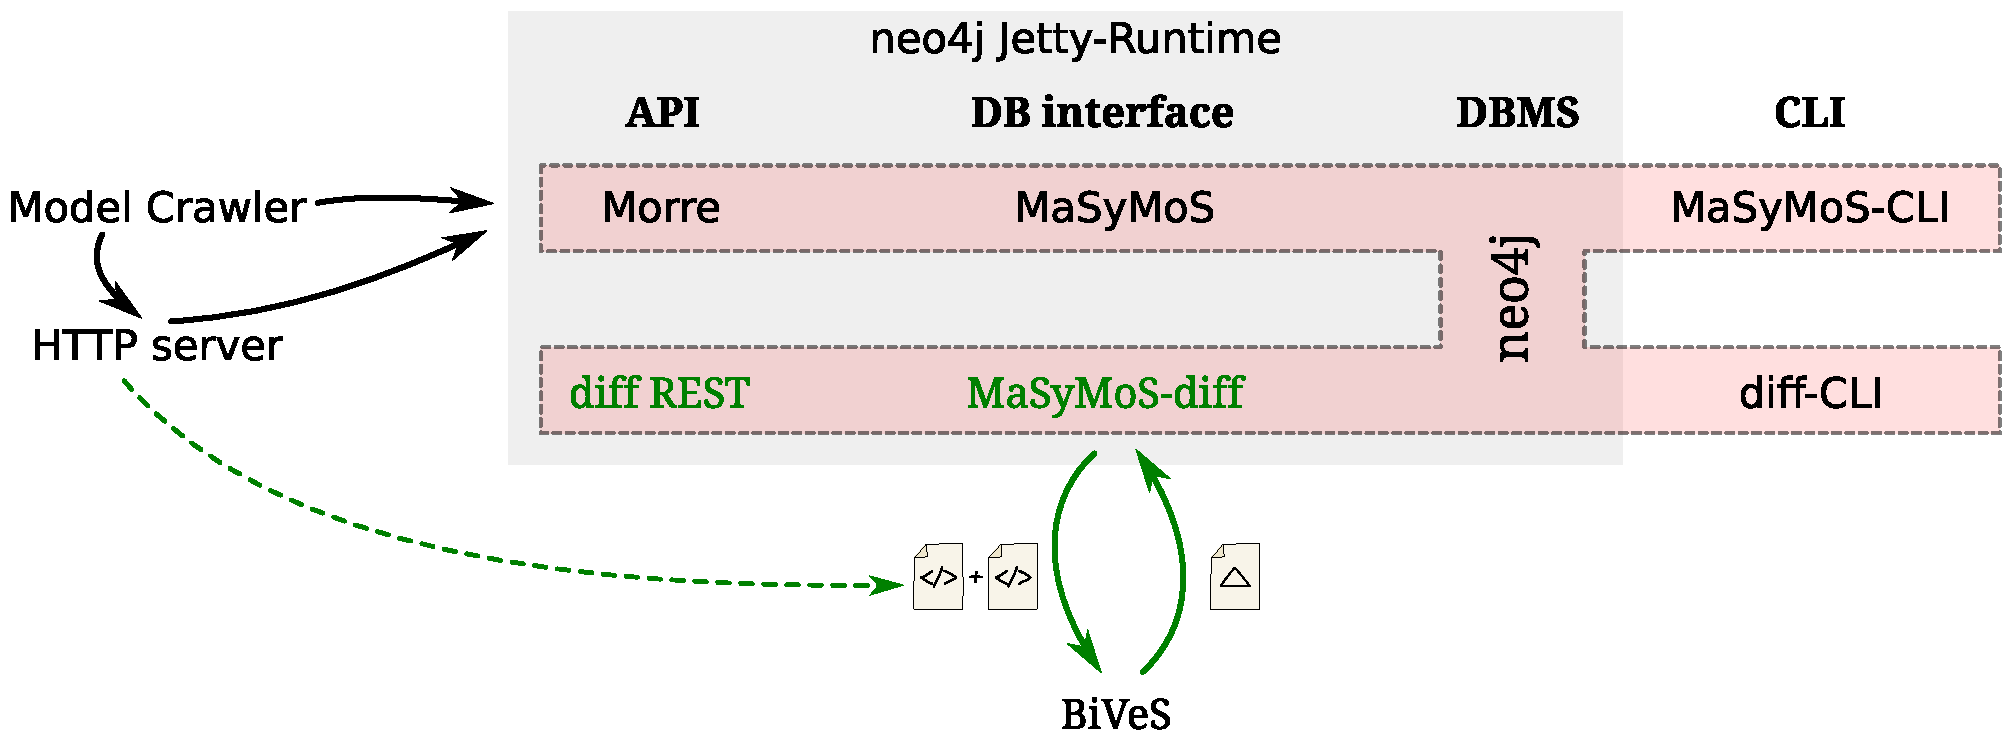
\includegraphics[width=\textwidth]{resources/system-overview-matrix.pdf}
	\caption{Infrastructure overview}
	\label{fig:system-overview}
\end{figure}

\section{Database model and storage decisions}
\begin{itemize}
\item extension to database model cf. \ref{fig:db-model}
	\subitem linking version
	\subitem storing differences
\item decisions on storage model
	\subitem storing each version full (no delta-storage)
	\subitem each version is aware to the search index
	\subitem diff still enables for analysis of changes
	\subitem higher storage consumption
\item extended storage model
\end{itemize}

% description of ER model
Figure \ref{fig:db-er-model} shows the proposed database schema as ER model. To reduce complexity and redundancy, for some entities only classes of higher hierarchy are modeled. E.g. a \texttt{DiffEntry} could be a \texttt{DiffInsert}, \texttt{DiffDelete}, \texttt{DiffModify} or \texttt{DiffMove}. Same applies for \texttt{ModelEntityType} and \texttt{ModelEntity}.
On the left hand side the model shows the existing structure, developed with \masymos. The entities and relations shown on the middle and right hand side shall be added in to process of prototype development.
\todo{Add color to the diagram, to ease explanation}
\todo{Find out, to what a Diff can link}

The schema is build around a \texttt{Diff} entity linking two \texttt{Document} entities, which are representing an (XML-)document containing a model. This entity does not necessarily need to span between two consecutive versions, but I decided for a standard setup it might be less useful to store differences between every possible combination of versions, since it would consume unreasonable amount of storage. Further are diffs concatable, so it does not take any computational effort to generate a diff for larger version steps out of consecutive diffs.

Every \texttt{Diff} entity links to multiple \texttt{DiffEntry} entities via the \texttt{has\_entry} relation. Each \texttt{DiffEntry} represents a difference detected by \bives \cite{Scharm2015}. Not modeled in the ER model is the differentiation between possible types of the diff (insert, delete, move, modify), which will be represented by using different additional label in \neoj.
Each \texttt{DiffEntry} links to at least on \texttt{ModleEntityType} or \texttt{ModelEntity} via either \texttt{old\_entity}, a \texttt{new\_entity}, or both, depending on the type of the difference.
For instance a \texttt{DiffInsert} links to a \texttt{ModelEntityType} or \texttt{ModelEntity} of \emph{Version B} with a \texttt{new\_entity} relation.
In contrast a \texttt{DiffDelete} links to \emph{Version A} with \texttt{old\_entity} to either a \texttt{ModelEntityType} or a \texttt{ModelEntity}. Whereby \texttt{DiffMove} and \texttt{DiffModify} use both relations \texttt{old\_entity} - linking to \emph{Version A} - and \texttt{new\_entity} - linking to Version B.

Additionally a \texttt{DiffEntry} can link to an \texttt{OntologyTerm}, which again can be hierarchical relating to another \texttt{OntologyTerm}. Those terms are taken from the \comodi ontology \cite{Scharm2016}, cf. section \ref{sec:background:comodi}.


\begin{figure}
	\centering
	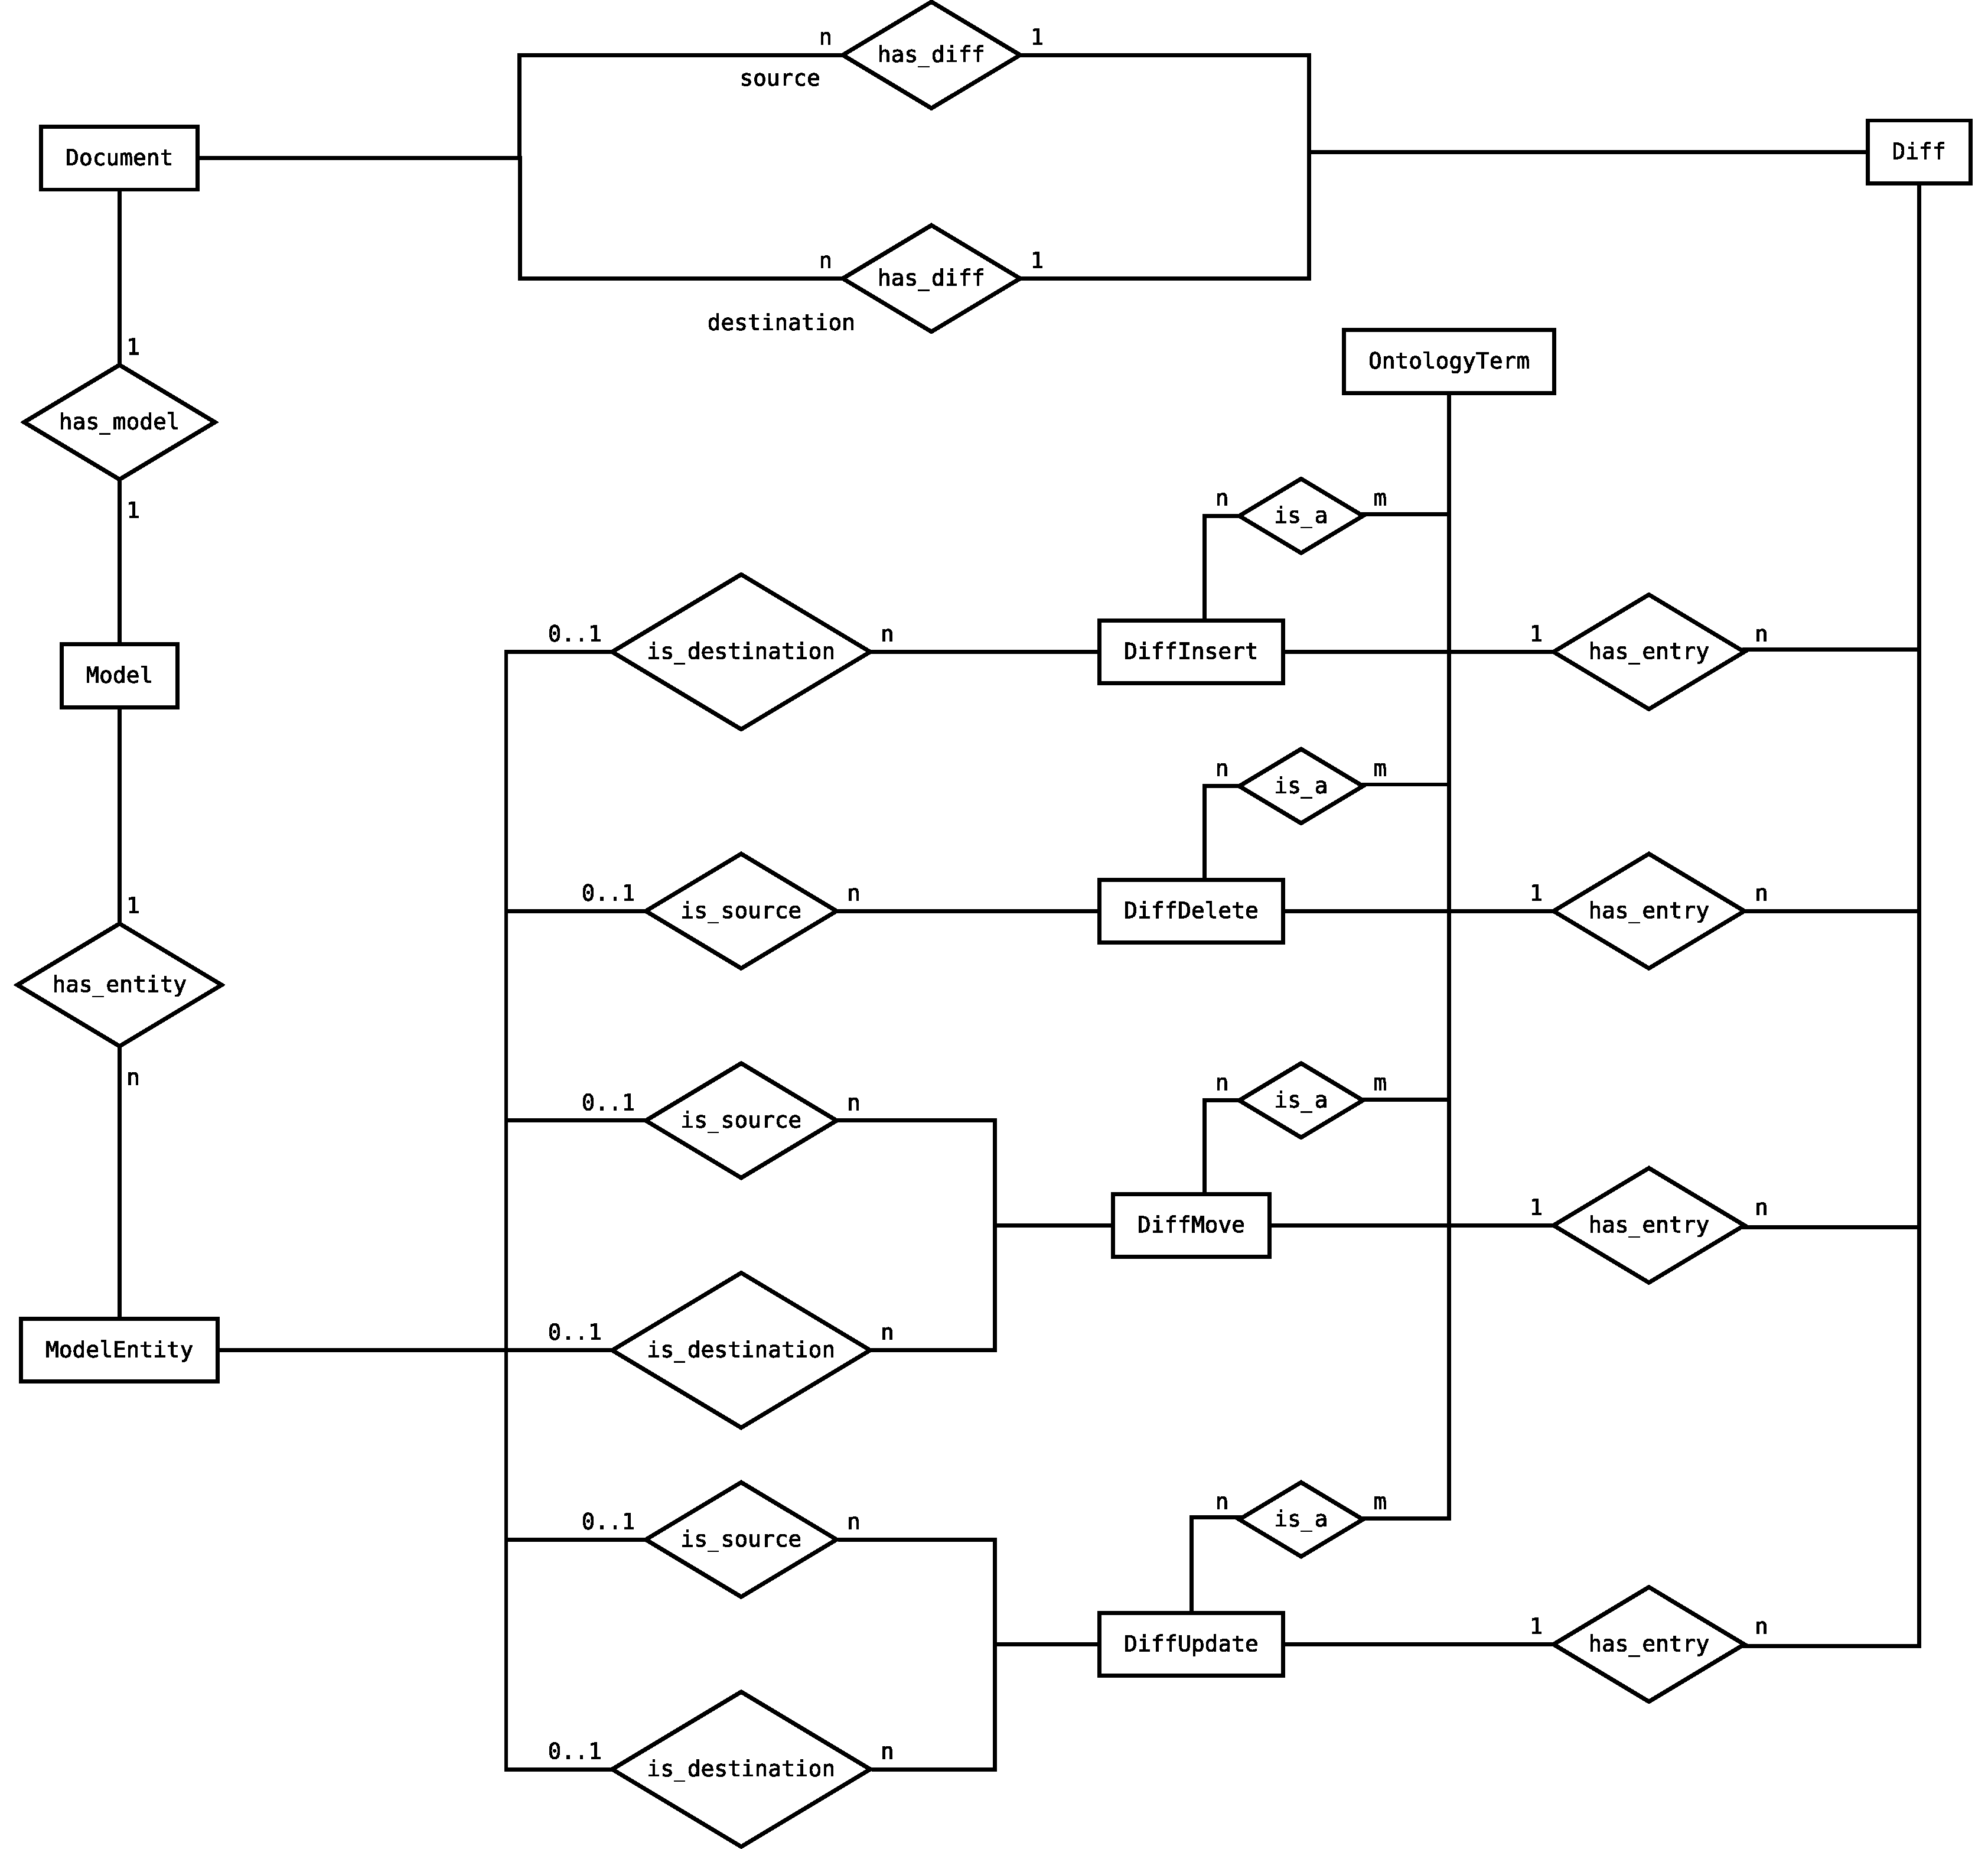
\includegraphics[width=\textwidth]{resources/db-concept-er.pdf}
	\caption{ER model of the proposed database schema}
	\label{fig:db-er-model}
\end{figure}

\begin{figure}[h]
	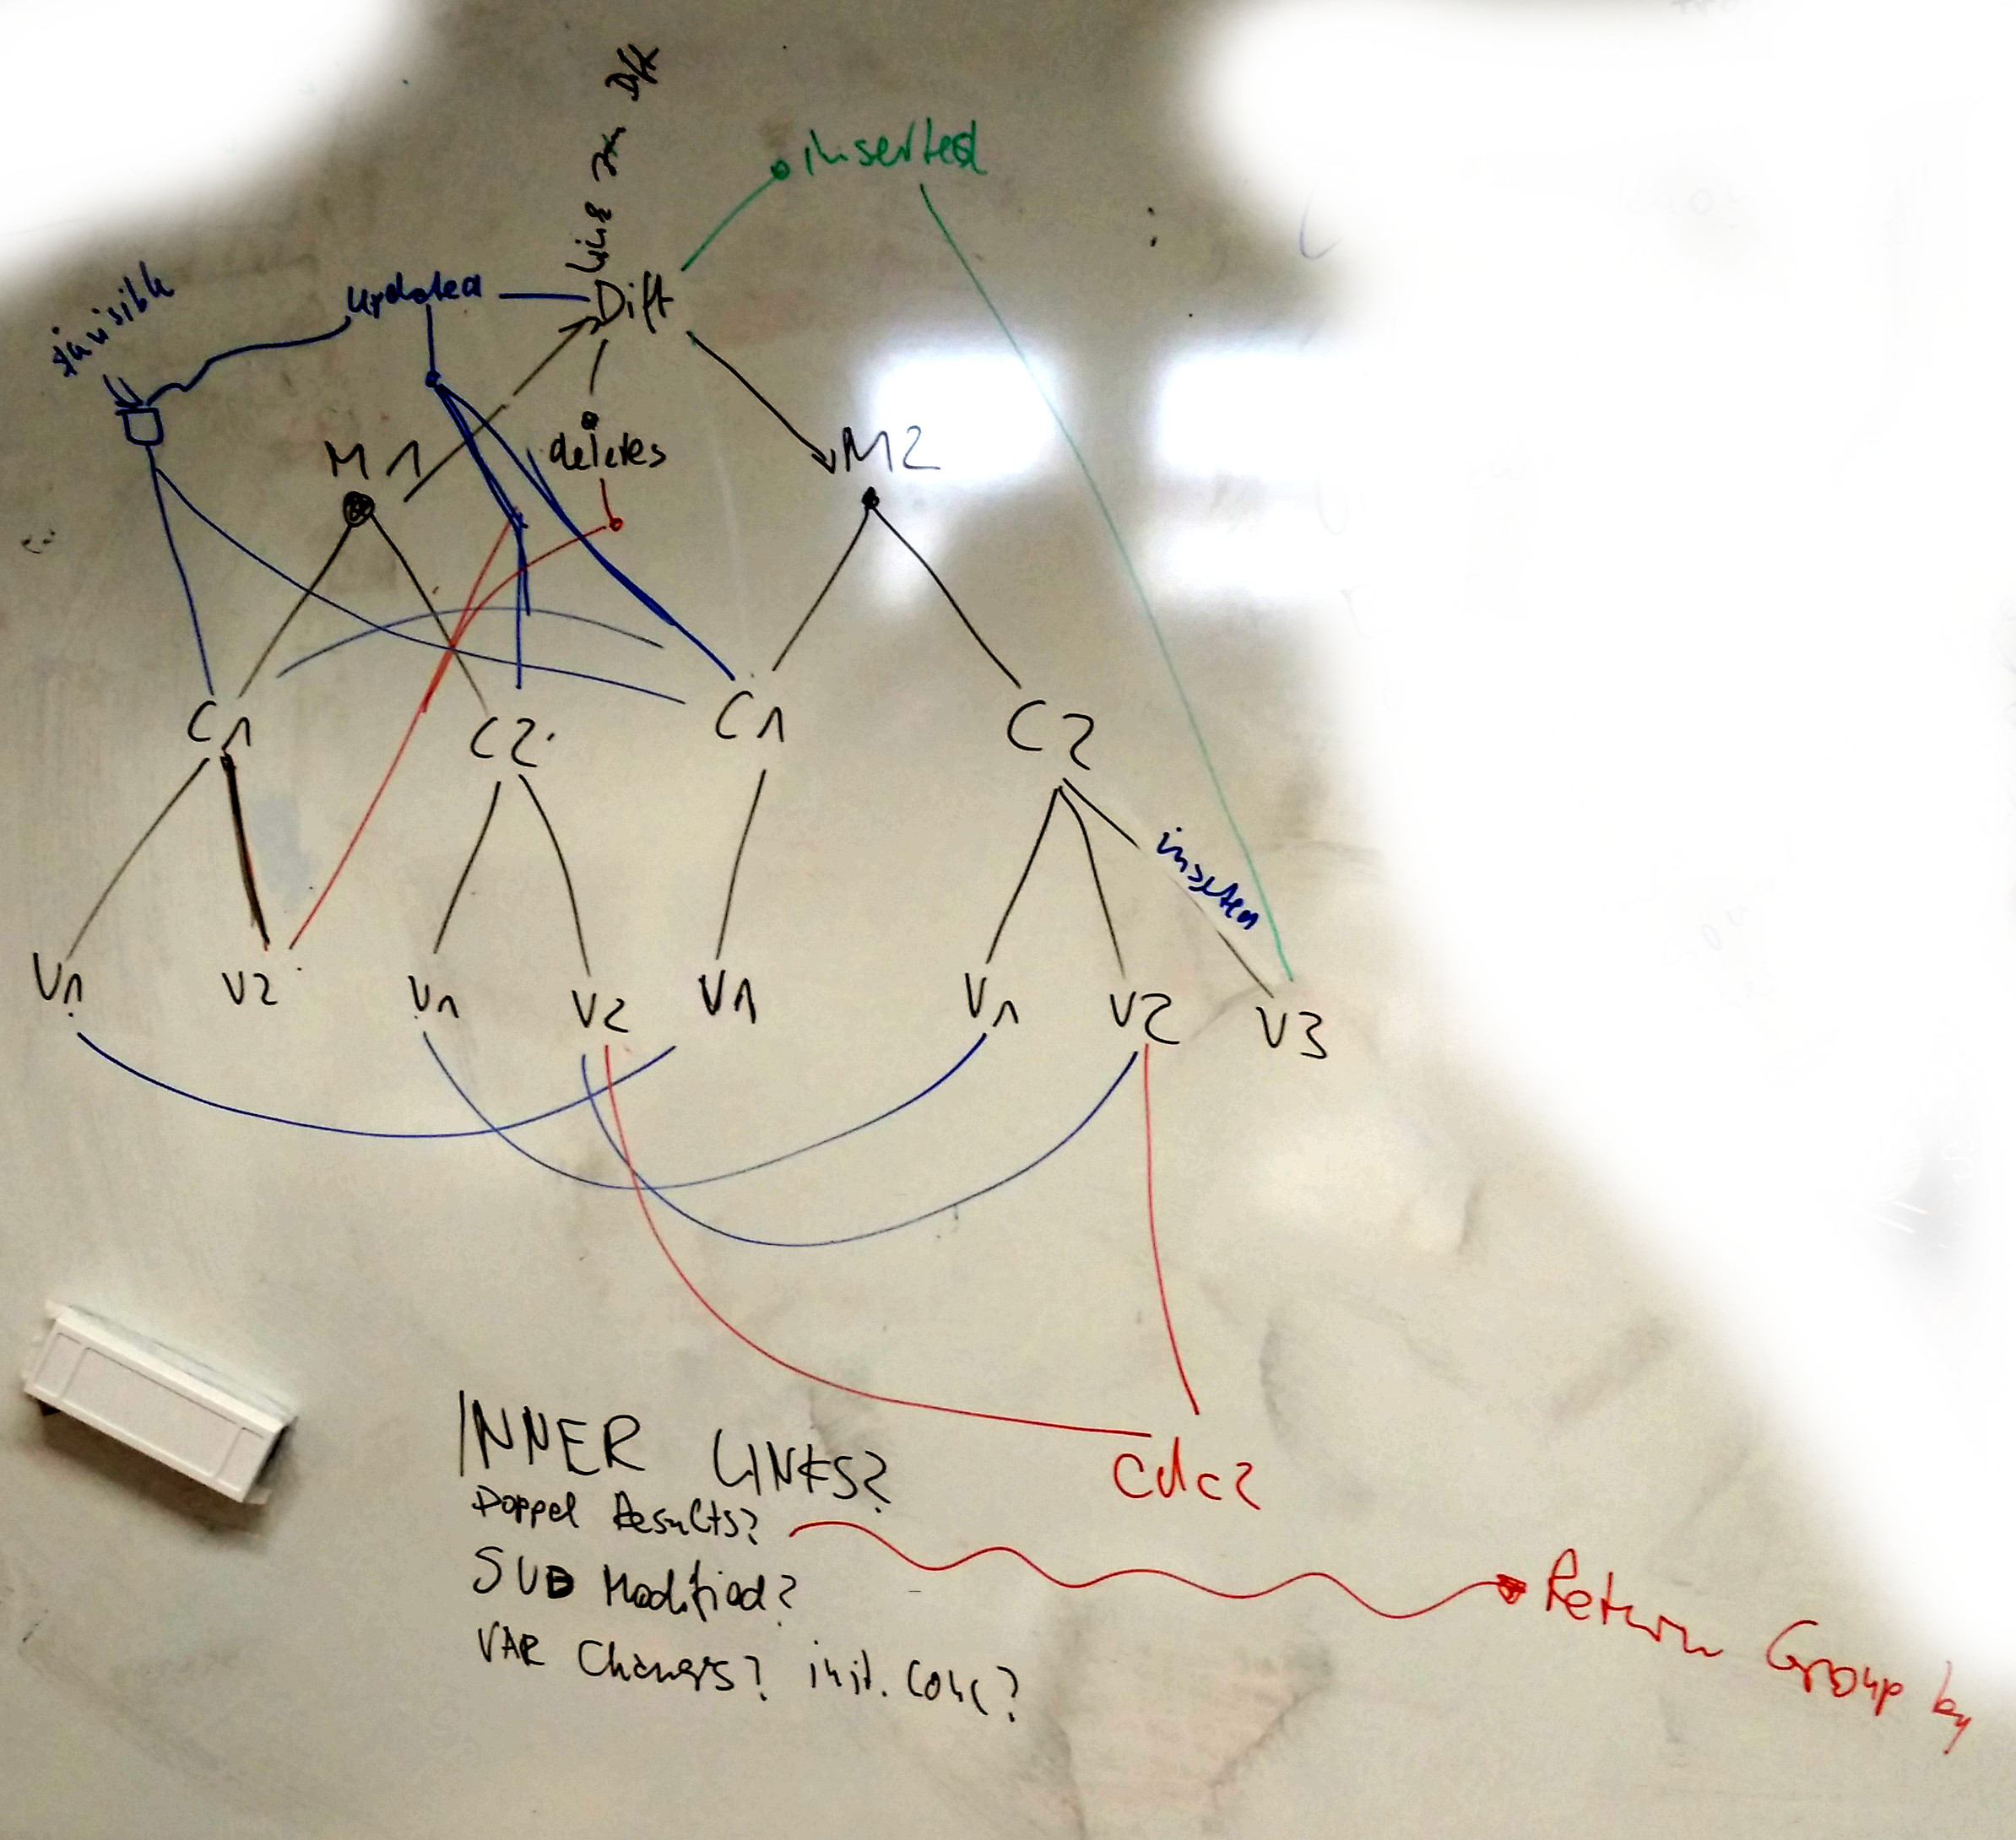
\includegraphics[width=\textwidth]{resources/db_structure.jpg}
	\caption{Proposed database structure}
	\label{fig:db-model}
\end{figure}

	
	\chapter{Results}
	% !TeX spellcheck = en_US
\label{sec:results}

Using the concept, described in Chapter \ref{sec:concept}, I was able to implement the newly designed parts of the ER model, shown in Figure \ref{fig:db-er-model}, in the \masymos \neoj stack. These graph structures are generated by a plugin written to interface the native \neoj API on the one side and \bives on the other.
Converting this formal described ER model into a graph database schema as shown in Figure \ref{fig:results:simple-diff}, was performed as described in Section \ref{sec:background:graph-db:er}. Despite the direct convertibility, some optimizations and adjustments for convenience were made, like introducing the common label \texttt{DIFF\_NODE} for all change types.
Also the figure shows a simplified representation of a delta between two versions of a relatively simple toy model. The figure was reduced to maintain readability, while still illustrating the basic schema.

The schema was designed around a \texttt{DIFF} node, which is linked by \texttt{HAS\_DIFF} relations, from two consecutive versions of the same model. These two versions are again linked with the \texttt{HAS\_SUCCESSOR} and \texttt{HAS\_PREDECESSOR} relations.
The successor and predecessor relations define the version history, whereby the \texttt{DIFF} node clearly indicates the delta between those versions. The \texttt{diffPart} attribute of the \texttt{HAS\_DIFF} relations specifies the direction of the delta, and therefore the role of the participating \texttt{DOCUMENT} nodes. In accordance to the ER model, the role can either be \emph{source} or \emph{destination}.
These terms were chosen, due to their expressiveness in regards to temporal aspects. Otherwise an implication of order, like terms as \emph{old} and \emph{new} suggest, may cause confusion in case of reverse deltas or deltas between completely different models.

However, the central \texttt{DIFF} node links to various changes, using the\linebreak \texttt{HAS\_DIFF\_ENTRY} relation. Since \neoj supports multiple labels per node, the four change types \texttt{DIFF\_INSERT}, \texttt{DIFF\_DELETE}, \texttt{DIFF\_UPDATE}, and \texttt{DIFF\_MOVE} can be grouped together using an additional label \texttt{DIFF\_NODE}. This simplifies queries and will eventually speed them up, because all change types are kept in a single index.
Any kind of \texttt{DIFF\_NODE} might link to any node beneath the \texttt{DOCUMENT} node in at least one of the two compared models, in correspondence to the type of change.
As illustrated by the \texttt{DIFF\_UPDATE} node in Figure \ref{fig:results:simple-diff} (small yellow node, labeled with a \emph{2}). On one hand it connects to the species \emph{A} in the \emph{source} version of the model using the \texttt{IS\_SOURCE} relation. On the other hand it also connects to the updated counterpart in this case species \emph{A} in the \emph{destination} version. It is connected using the \texttt{IS\_DESTINATION} relation.
Furthermore a causality chain among changes is expressed by the \texttt{DIFF\_TRIGGERED\_BY} relation, which points from one \texttt{DIFF\_NODE} to another. This is illustrated by the \texttt{DIFF\_INSERT}, labeled with the number \emph{3}, in Figure \ref{fig:results:simple-diff}. This insert caused four other inserts, describing the insertion of id, name, compartment reference, and initial concentration.

In addition to these structural information each \texttt{DIFF\_NODE} contains all attributes \bives assigns to a change. These \bives specific information include an XPath expressions, name, and id of the changed \xml element. All these attributes can be used together, to locate the change in both versions.
Further the nodes includes the values of \emph{source} and \emph{destination} in case of an attribute change, as well as a possible reference to another change, that triggered this current one.
Besides the \bives attributes, the \texttt{DIFF\_NODE} also contains an \texttt{inherit} flag. It indicates, if a change detected by \bives, does not have a direct match in \masymos's graph structure. Instead the model structure is traversed upwards, until an element is found, which has a representation in the \masymos graph.
This, for instance, applies to changes of a mathematical parameter in a kinetic law of a reaction. In this specific example, the change would be linked to the node representing the reaction, since mathematical structures or kinetic laws are not represented in \masymos. Another example would be text nodes of any kind, which are stored within a Lucene index by \masymos, but not in the graph representation, since they are not an essential part of the models structure.
The \texttt{inherit} flag consequently allows to store and analyze changes, which otherwise could not be integrated into the schema.

Furthermore \texttt{DIFF\_NODE} nodes might link to multiple \comodi terms, whereby \comodi's own relationship names are used, instead of the generic \texttt{is\_a} link, proposed in the concept Section \ref{sec:concept:dbmodel}.
Further \comodi's entire reasoned taxonomy is stored in \masymos, so queries matched against abstract terms also include references to more specialized terms. The resulting network is shown in Appendix \ref{fig:appendix:neo4j-comodi}.
Before generating any deltas the \comodi ontology needs to be imported initially. Otherwise terms might be created on occurrence, but not interlinked according to the taxonomy.
The initial import is performed using already existing mechanisms in \masymos, which were only adjusted, so they can handle dynamic ontology names (cf. Section \ref{sec:impl:masymos}). In this process the ontology is first loaded in its \owl representation and then validated with the Hermit reasoner \citep{Shearer2008}. The second step does not only makes sure that only logically correct ontologies are imported, but also to imports \emph{inferred} ontologies. This moves the logical classification step from querying to the import of ontologies.
A graphical and tabular overview of all used node labels and relation types can be found in Appendix \ref{sec:appendix:meta-map}.

The import of actual models, however, is performed by the \modelcrawler (cf. Section \ref{sec:impl:modelcrawler}), resulting in a \masymos database filled with all model versions of \emph{BioModels Database} and \emph{PMR2} (cf. Section \ref{sec:background:modelrepo}) and a hierarchical file structure containing all original files, complying with the model described in Section \ref{sec:concept:filestorage}.
During a test run from 2016-10-14, this resulted in a dataset with $3367$ distinct models and  $14503$ model versions, with $4.307$ versions per model on average. The accumulated test data consumes $8.5$ GBytes of disc storage for the database, excluding the cached original files (cf. Section \ref{sec:concept:filestorage}).
This data was gathered from all publicly available workspaces in \emph{PMR2} and all releases of the \emph{BioModels database} (cf. Section \ref{sec:background:modelrepo}) using the \modelcrawler (cf. Section \ref{sec:impl:modelcrawler}).
\todo{point to appendix, explaining how the import was done}

On the contrary, models for test purposes and to generate Figure \ref{fig:results:simple-diff} were imported using a small Python\footnote{\url{https://www.python.org/}} script. This script emulates a HTTP daemon, while simultaneously sending import commands to the \masymos \rest interface \morre. It eases the process of importing test data, since neither the \modelcrawler needs to be configure, nor a sane folder structure needs to be built manually.

In conclusion, the extension of the \masymos database allows to store, access, query, and compare multiple versions of biological models, enriched by semantical annotations. Whereas the extended \masymos database is providing an efficient index for a variety of structural, textual and semantic aspects, the original files are still available in the filesystem.
This attempt combines benefits from both approaches.
On one hand the indexed graph database provides excellent analytical features while maintaining reasonable performance. On the other hand it ensures the exact reproduction of the original model files.
Overall this solution meets the requirements set by \citet{Waltemath2013}, that a good "model VCS should be tailored to existing model  representation formats, which are typically XML and RDF based. It should furthermore reflect the temporal evolution of a model and present model changes to the users" \citep{Waltemath2013}.

\begin{figure}[h]
	\centering
	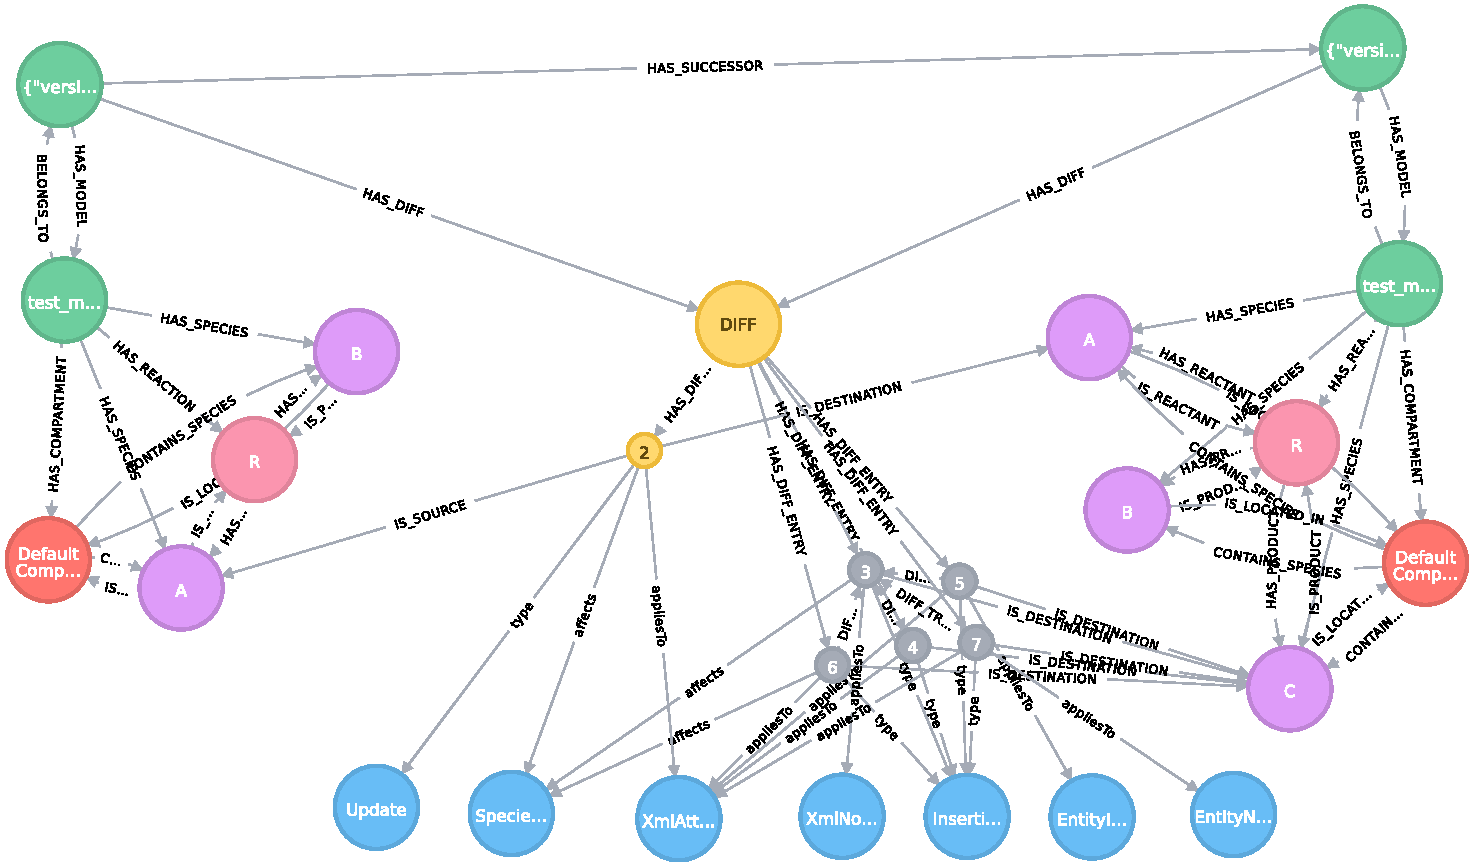
\includegraphics[width=\textwidth]{resources/neo4j-renders/demo-sbml-simple-diff.pdf}
	\caption[Reduced representation of a delta in \masymos, between two versions of a the simple \sbml demo model]{Reduced representation of a delta in \masymos, between two versions of a the simple \sbml demo model. The delta, organized around the \texttt{DIFF} node shows only changes with a direct match in the graph representation. Further most up traversing relations are not shown, to increase readability.
		The small nodes are \texttt{DIFF\_NODE} representing either inserts (green) or a update (yellow) in this example. A full version can be seen in Appendix \ref{fig:appendix:demo-sbml-simple-diff}}
	\label{fig:results:simple-diff}
\end{figure}
 
\begin{comment}
\todo{what's done from the concept}
\todo{still high-level}
\todo{what problem is solved?}

\begin{itemize}
	\item implemented db concept
		\subitem picture from simple-sbml-demo
		\subitem rest of pictures in appendix
	\item Ontology import
		\subitem changes to \masymos core
		\subitem using existing import mechanics, but dynamic
	\item http server storage concept?
\end{itemize}

solved:
"A model VCS should be tailored to existing model representation formats, which are typically XML and RDF based. It should furthermore reflect the temporal evolution of a model and present model changes to the users." \citep{Waltemath2013}

The objective of this thesis is therefore to investigate into a concept to store systems biology models in a way, that multiple versions can be accessed, queried, and compared. Further, semantical annotations of changes between these versions shall be introduced. These additional relations are meant to improve the ability to query for a version of a model by specific criteria and consequently improving the user experience for biologists seeking to build onto existing models, as the evolution of them plays an important role for them \citep{Scharm2015}
\end{comment}
	
	\chapter{Implementation of the Prototype}
	% !TeX spellcheck = en_US
\todo{concrete, low-level stuff}
\todo{what was used, version numbers, etc.}
\todo{pretty short, every subproject gets a section}
\todo{add figure showing differences of concept and implementation, regarding figure \ref{fig:system-overview}}

\section{\modelcrawler}
	\label{sec:impl:modelcrawler}
	The \modelcrawler is not a direct product of this project, but was developed by me in course of my work as student assistant at the department for \sysbio and Bioinformatics. However, it is mentioned here, since it responsible for creating the repository containing all original files, which is one of the integral parts of the presented concept (cf. Section \ref{sec:concept:filestorage}).
	
	The version described here is 0.0.4 mark2, commit \texttt{abb63db}. Overall the function of the \modelcrawler is relatively simplistic and was designed, so it could be ran incrementally, gradually crawling only (a limited amount) new versions. Each pass through therefore consists of two steps: First the databases are crawled, the new versions or releases are downloaded and stored in said file structure.
	Second the \modelcrawler pushes all new model versions to \masymos, theoretically allowing for improved write speed, due to transaction management. However, the main reason for splitting the actions is better error recovery. By keeping the time of write operations on the database short and not running any other concurrent task, the probability of interruptions is minimized. This means, when the \modelcrawler fails, due to bugs in the implementation, changes in the API, or other external influences (e.g. Java Heap Exceptions), the database does not get inconsistent. This is guaranteed, because ahead of inserting data, the \modelcrawler ensures all data is valid and consistent.
	
	However the first step, downloading all new versions, depends heavily on the intended database.
	In case of \emph{BioModels Database} all unknown/new releases are downloaded from the FTP server with Apache Commons Net library version 3.3, unpacked with the Apache Commons Compress version 1.9. Consequently each \xml file is analyzed.
	If a file is already indexed in \masymos, the SHA-1 hash of the files is calculated. If this differs from the file hash of the latest version in \masymos, a new version is assumed. The files are distinguished by their name, which is equivalent to the \emph{BioModels ID}.
	
	This process is easier for \emph{PMR2}, since it already uses git repositories to keep track of versions/revisions of models. Therefore it is just a matter of interfacing the \rest API with Apache HttpClient 4.3 and FasterXMLs Jackson 2.5.1, to list all publicly available repositories. These repositories are then cloned or pulled with eclipses JGit library, version 3.7.0. Following all commits are iterated, and all newer than the latest version in \masymos are considered new.

	Since the \modelcrawler relies on the \masymos database, to identify already existing versions, it can operate stateless between different pass throughs. However, it keeps separately track of already downloaded BioModels releases and all previously cloned git repositories in order to minimize the amount of data, which needs to be transfered.

\section{Extension to the \masymos core}
	\label{sec:impl:masymos}
	\todo{add version number and commit hash}
	The anatomy of the \masymos project is divided into 3 parts: a core, a command line interface, and web \rest interface (cf. Section \ref{sec:background:graph-db:masymos}). This project was designed to mimic this structure, so modifications to the original implementation of \masymos ca be kept minimal. Due to the additive nature of the database concept (cf. Section \ref{sec:concept:dbmodel}), this design constraint could be met, except in one case.
	
	The only direct extension of the core implementation concerns the import of ontologies. By default \masymos allows to load a hard coded set of ontologies, which unfortunately does not include \comodi. Therefore I needed to extend \masymos for this capability. But instead of adding another name to list, I rather implemented a dynamic unique factory. The way \masymos handles ontologies features in particular node label indexes for each ontology, which is used as reverse index to ensure uniqueness of nodes representing a specific term.
	The benefit of this approach is, that even when an ontology is not yet imported, but a model or delta uses certain terms, these are created on demand. Later, when said ontology is loaded, the term representing nodes already exist and can be reused and correctly interconnected.
	The new method I have implemented, now allows to create other dynamic unique factories at runtime, effectively allowing to import any ontology.

	\begin{comment}
	\begin{itemize}
		\item generic ontology import for COMODI
		\item some helper methods/functions
	\end{itemize}
	\end{comment}

\section{\masymos diff plugin}
	\label{sec:impl:diff}
	As mentioned above (cf. Section \ref{sec:impl:masymos}) the implementation structure of this project is meant to mimic the one of \masymos. Hence the main logic is implemented in a core, which possibly gets extended by multiple interfaces (cf. Section \ref{sec:impl:rest}).
	
	This core implementation is designed to operate completely asynchronous, which makes the \texttt{ThreadPoolExecutor} a central part of this implementation. This executor is fed by a priority queue, allowing to prioritize urgent tasks, which may be blocking in terms of user interaction.
	Generally 3 tasks are implemented. First the \texttt{DiffGatherTask}, traverses through the database and submits \texttt{DiffGenerationTask}s for every version hop, not already connected by a delta.
	Secondly the \texttt{DiffGenerationTask} generates the actual delta with \bives and inserts its node representation into the database, using a single transaction.
	Third the \texttt{DiffCleanTask} can be used to remove all existing diffs from the database, which is especially useful during development and testing, but also when \bives is updated, since newer versions might improve detection of  change and annotation of them.
	
	In the current version this implementation uses the \bives library in version 1.9.1. Initially it was planned to rely on the \bives web service, because this is easier to update and would allow for better load balancing in large installations.
	This design decision was changed, because the translation of the \bives \xml output into an interlinked graph representation requires profound knowledge of both compared models. To create a mapping of the XPath expressions from \bives to the actual \xml elements of the model and consequently to nodes in \masymos, the capability of \bives to decode these model files is used. Since the decoding and document tree parsing is also essential for the generation of deltas in \bives (cf. Section \ref{sec:background:diff:bives}), externalizing the delta computation would therefore lead to unnecessary redundant processing and accordingly increase the computation time.
	
	A major issue is occurred in reliability tests of large transactions on the graph database. The origin of this problem lies \neoj's transaction management. Due to the memory consuming nature of graph storage and operations, large transactions may fail, because the Heap Space of the Java Virtual Machine (JVM) was exceeded. Especially the cleaning task suffered from this problem, but also the main \texttt{DiffGenerationTask} did.
	The space consumption of the \texttt{DiffGenerationTask} could be handled by increasing the maximum assigned memory of the JVM. Whereas it was necessary to modify the \texttt{DiffCleanTask} so it uses multiple smaller transaction per pass through.
	
	\begin{comment}
	\begin{itemize}
		\item interaction with \bives and neo4j
		\item problems with Transaction rollback in actually successfull transactions
		\item trigger for generating diffs for new versions
	\end{itemize}
	\end{comment}

\section{\rest interface}
	\label{sec:impl:rest}
	
	To interact with the diff plugin a \rest interface was implemented, similar to \masymos's \morre. It is realized as a unmanaged \neoj extension\footnote{\url{http://neo4j.com/docs/java-reference/current/\#server-unmanaged-extensions}}. As the \neoj manual suggests, it uses JAX-RS\footnote{\url{https://jax-rs-spec.java.net/}} 2.0 to define interfaces and Jackson\footnote{\url{http://wiki.fasterxml.com/JacksonHome}} 2.3.3 to serialize Java objects into \json.
	
	The \rest interface provides 4 endpoints to interact with, either triggering the \texttt{DiffGatherTask} or the \texttt{DiffGenerationTask}, or to enquire some basic statistics of the \texttt{ThreadPoolExecutor} or the database status in terms of generated deltas.
	The thread pool statistics include the number of queued tasks, currently executed tasks, and the immediate running tasks.
	However, the database statistics show the number of \texttt{Diff}s, \texttt{DOCUMENT}s, versions per distinct model, and the distribution of the different types of changes.
	
	\begin{comment}
	\begin{itemize}
		\item \rest interface for requesting diffs
	\end{itemize}
	\end{comment}
	
	\chapter{Discussion}
	\todo{}
\begin{itemize}
	\item Benchmarks/stats on database
		\subitem additional overhead (nodes/relations increase)
	\item How to improve database/reduce overhead
	\item 2 branches of \comodi unused
		\subitem because of automatic generation
		\subitem reason and intention not able to be automatically determined
		\subitem possible extension?
\end{itemize}

	
	\chapter{Outlook}
	\begin{comment}

\begin{frame}[t]{}{\mylogo}\vspace{-1em}
{\textcolor{colorscheme} {\textbf{That's it!}}}\\
\begin{tikzpicture}[>=stealth',trans/.style = {->,densely dashed,lightgray},shift={(-3,-3)},font=\small\selectfont]
\node[anchor=west] (sems) at (0,0) {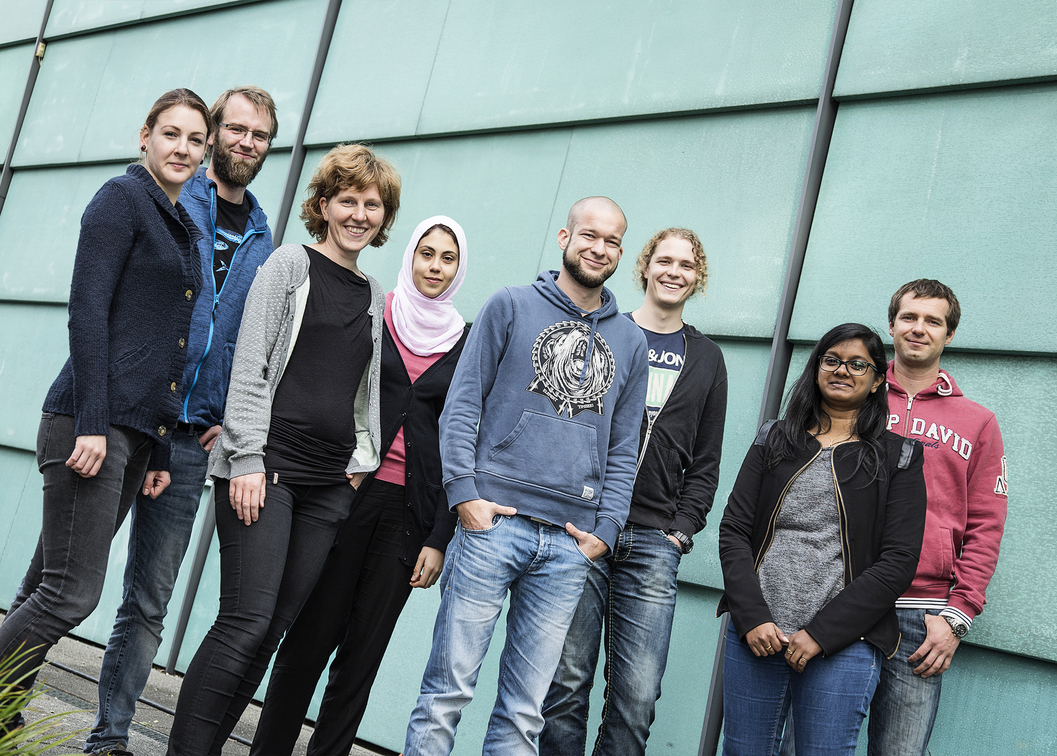
\includegraphics[height=.55\textheight]{res/group-2016.jpg}};
\node[anchor=west] (jws) at (4.9,0) {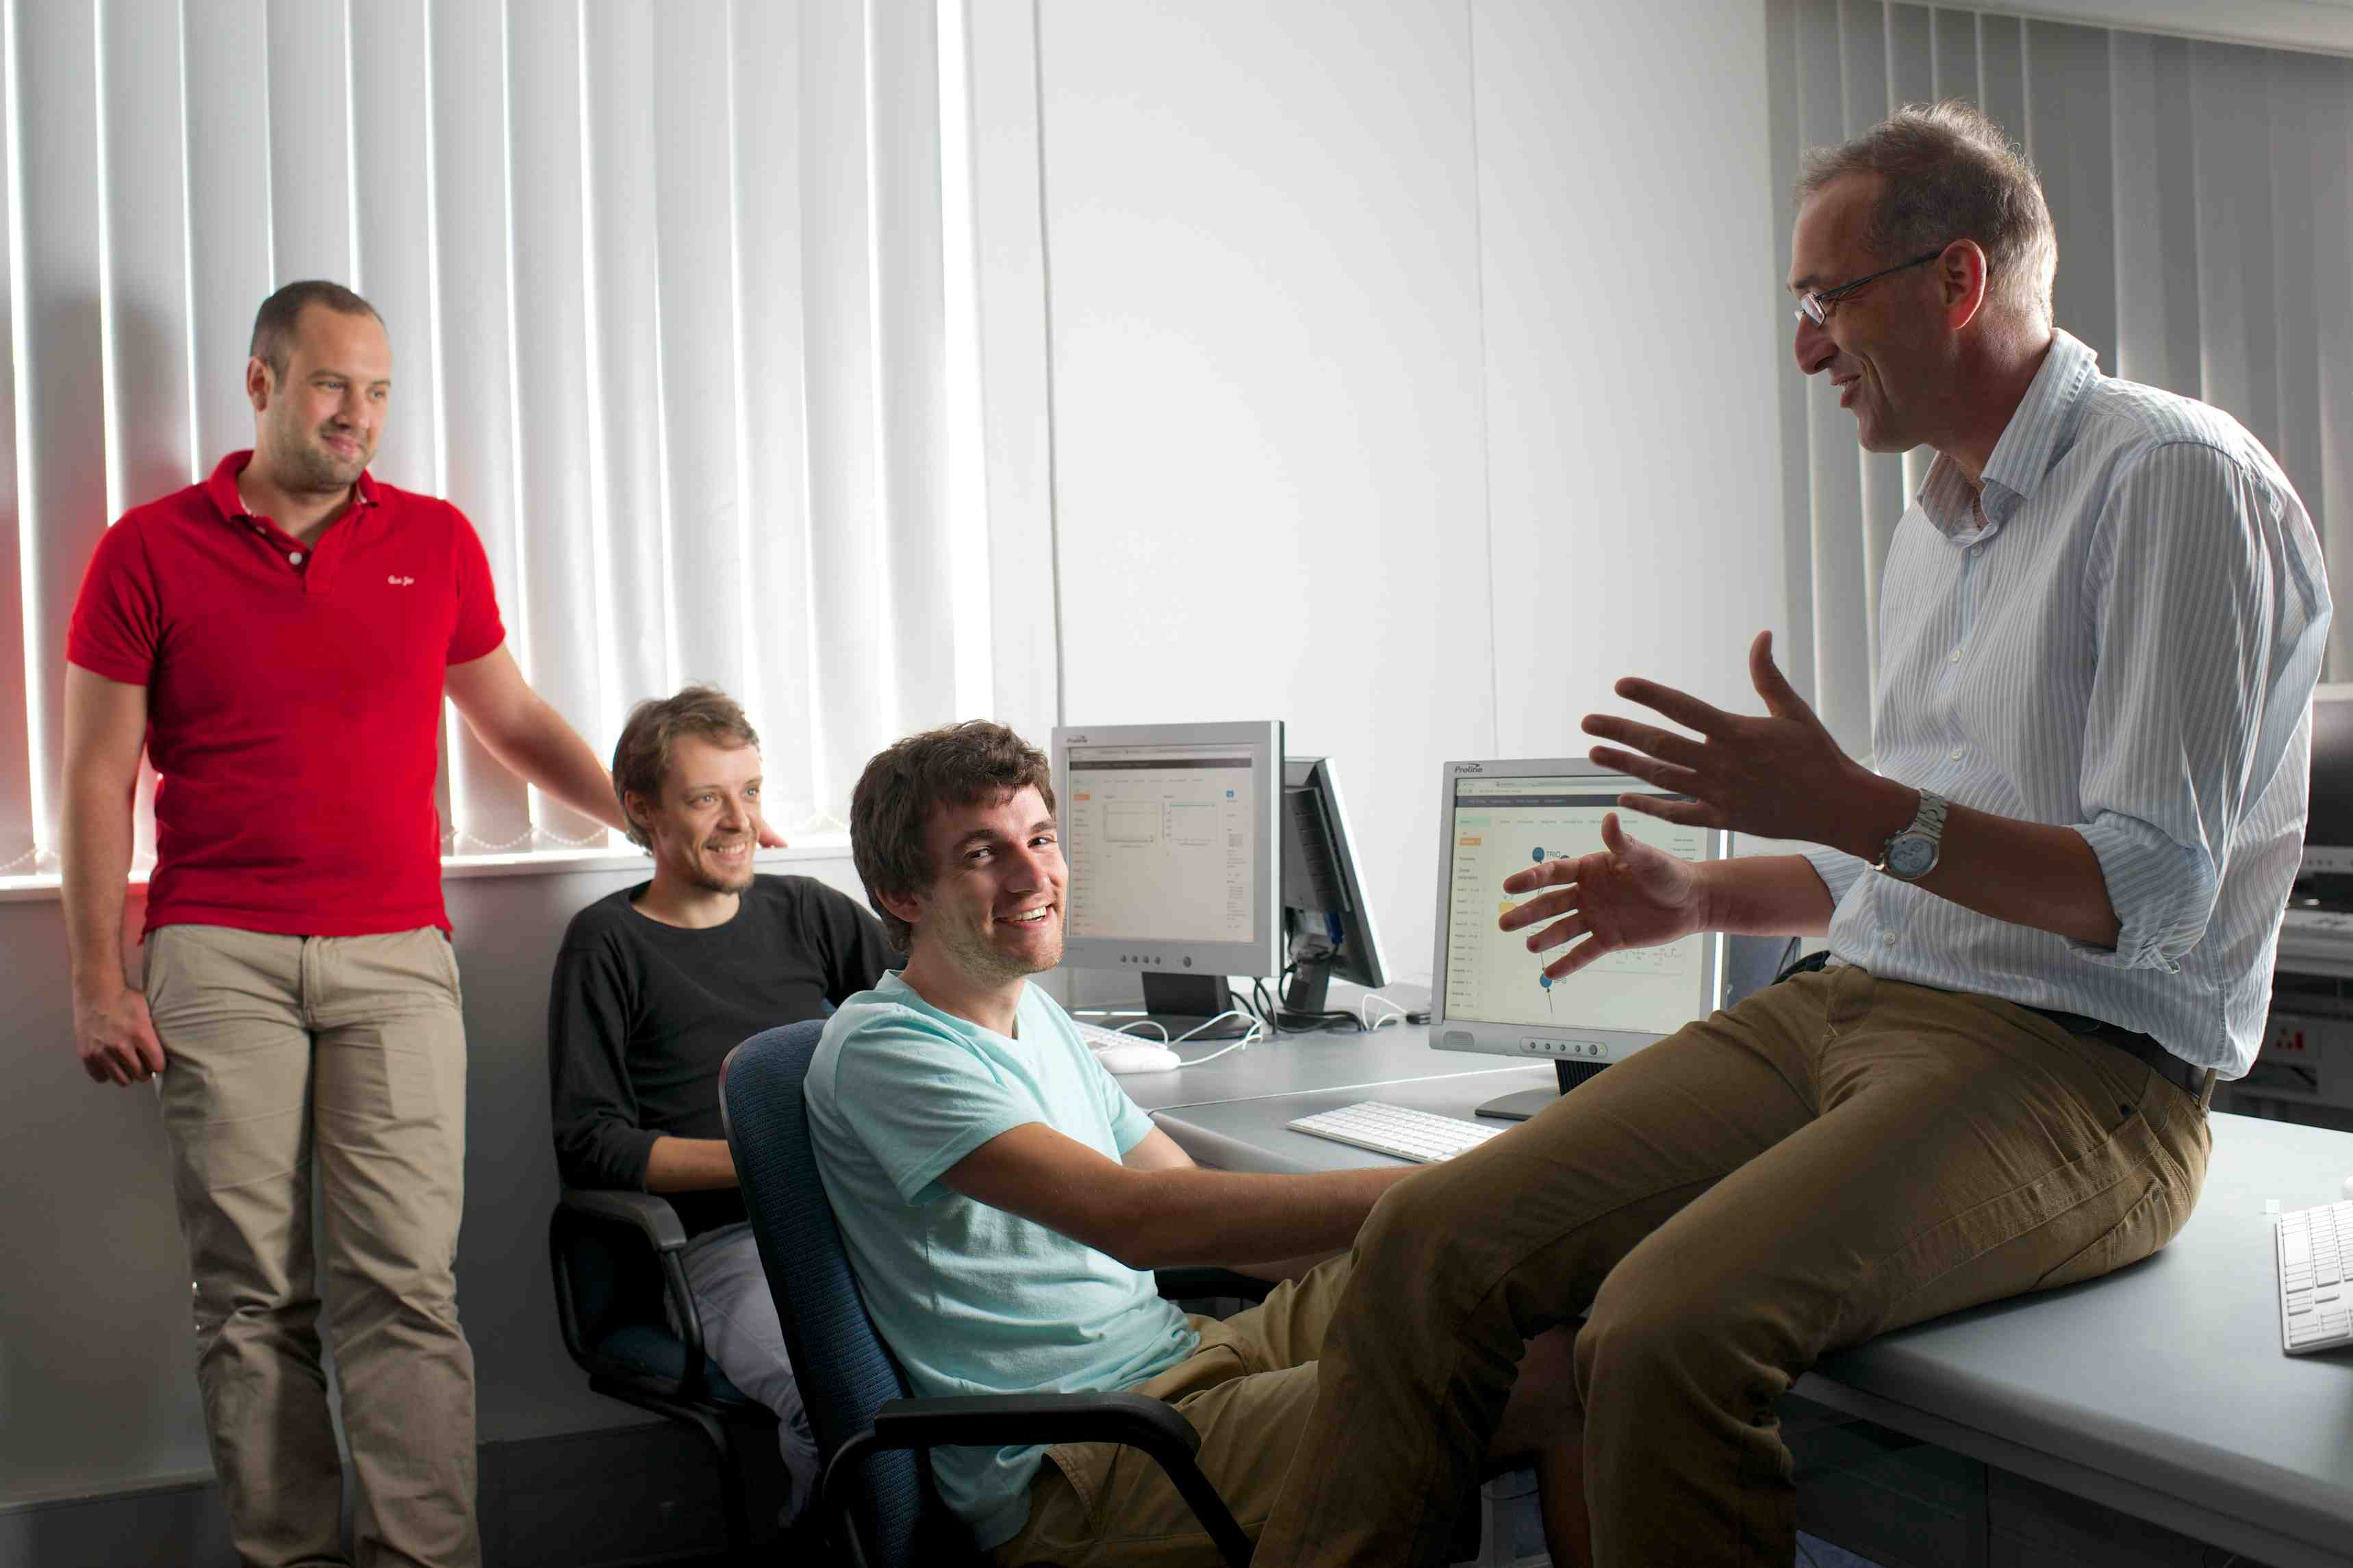
\includegraphics[height=.55\textheight]{res/jws_team.jpg}};
\node[yshift=-.1cm] at (sems.south) {SEMS Task Force};
\node[yshift=-.1cm] at (jws.south) {JWS Team};

\node[anchor=west] at (0, -3.45)  {
	\begin{minipage}[t][][t]{0.25\textwidth}
		\footnotesize
		Fabienne Lambusch\\
		Martin Scharm\\
		Dagmar Waltemath\\
		Mariam Nassar\\
	\end{minipage}
};

\node[anchor=west] at (2.7, -3.3)  {
	\begin{minipage}[t][][t]{0.25\textwidth}
		\footnotesize
		Tom Gebhardt\\
		%Martin Peters\\
		Vasundra Toure\\
		Ron Henkel\\
		Olaf Wolkenhauer
	\end{minipage}
};

\node[anchor=west] at (5.4, -3.32) {
	\begin{minipage}[t][][t]{0.25\textwidth}
		\footnotesize
		Dawie van Niekerk\\
		Johann Eicher\\
		Daniel Palm\\
		Jacky Snoep
	\end{minipage}
};

\node[anchor=west] at (9, -3.5) {
	\begin{minipage}[t][][t]{50pt}
		\hfill {\tiny funded by}\\
		\centering
		\includegraphics[width=50pt, height=2.5em, keepaspectratio]{res/BMBF-Logo.pdf}\\
		
\includegraphics[width=50pt, height=2.5em, keepaspectratio]{res/NRF_logo.jpg}
	\end{minipage}
};

\end{tikzpicture}

% % \scriptsize
% \begin{minipage}[t][.6\textheight][t]{.4\textwidth}
% %\vfil
% \quad\begin{tikzpicture}[overlay]
%  \node[rotate=90] at (-.5,-1.3) {SEMS Task Force};
%  \node[rotate=90] at (-.5,-4.3) {SBI Team};
% \end{tikzpicture}\\
% 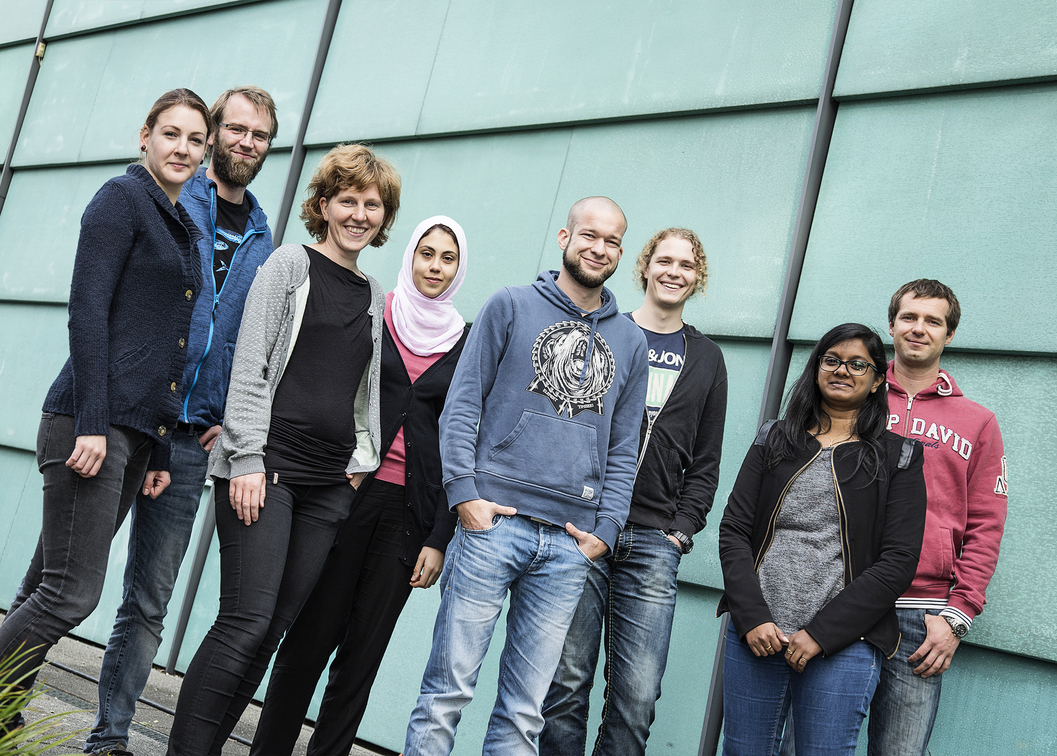
\includegraphics[width=.95\textwidth]{res/group-2016.jpg}\\[.5em]
% 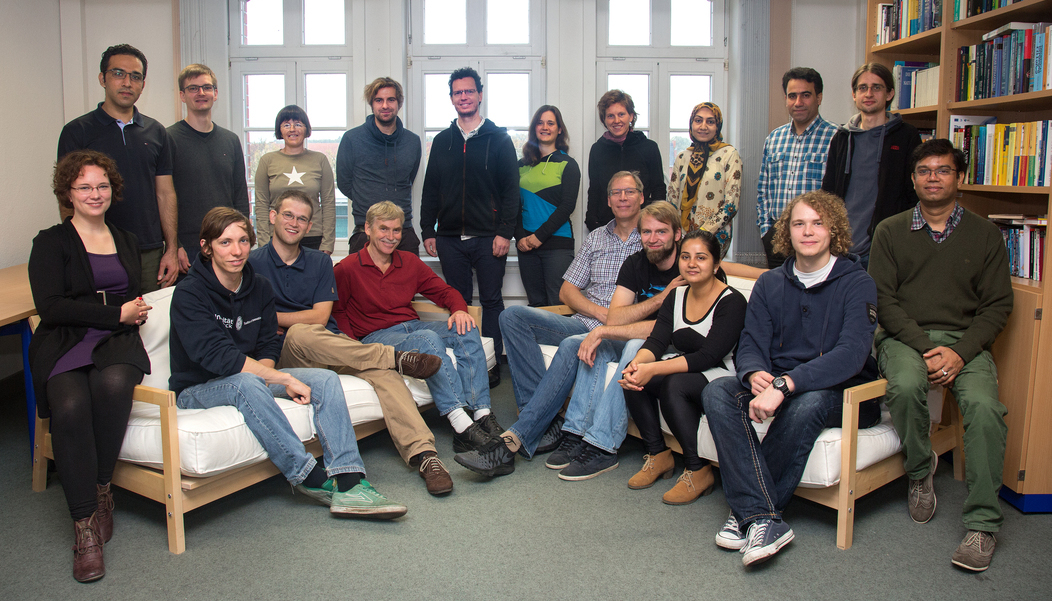
\includegraphics[width=.95\textwidth]{res/group-sbi.jpg}
% % \textbf{SEMS group}\\[.5em]
% % Dagmar Waltemath\\
% % Ron Henkel\\
% % Martin Peters\\
% % Markus Wolfien\\
% % Rebekka Alm\\
% % Olaf Wolkenhauer\\[1em]
% % \vfil
% % 
\includegraphics[height=1em]{res/twitter.png}\ \textcolor{colorscheme}{\tt\href{https://twitter.com/semsproject}{\small @SemsProject}}\\
% % \textcolor{colorscheme}{\tt\href{http://sems.uni-rostock.de}{\small http:\twobar{}sems.uni-rostock.de}}\\
% \vfil
% \end{minipage}
% % \hfill
% \begin{minipage}[t][.6\textheight][t]{.3\textwidth}
% % \vfil
% \quad\\
% % \textbf{SEMS group}\\[.5em]
% Tom Gebhardt\\
% Fabienne Lambusch\\
% Mariam Nassar\\
% Martin Peters\\
% Vasundra Toure\\
% Dagmar Waltemath\\
% Olaf Wolkenhauer
% % \textbf{SBI group}\\[.5em]
% % Olaf Wolkenhauer\\
% % Markus Wolfien
% \vfill
% \end{minipage}
% % \hfill
% \begin{minipage}[t][.6\textheight][t]{.29\textwidth}
% %\vfil
% %\textbf{Collaborators}\\[.5em]
% % Falk Schreiber\\
% % Jonathan Cooper (University of Oxford)\\
% % % COMBINE\\
% % \quad\\
% % 
\includegraphics[width=10em]{res/COMBINE.png}\\
% % 
\includegraphics[width=10em]{res/COMBINE.png}\\
% % 
\includegraphics[width=4em]{res/seek-logo-original.png}\hfill
% % 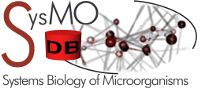
\includegraphics[width=6em]{res/sysmodb2.png}\\
% % 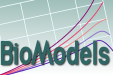
\includegraphics[width=5em]{res/bmdb.png}\hfill
% % \includegraphics[width=4em]{res/CellML-eps-converted-to.pdf}\\
% % \vfil
% \end{minipage}
% 
% \begin{flushright}
% 
\includegraphics[height=4em]{res/ptj-logo.png}\hspace{1em}\includegraphics[height=4em]{res/BMBF-Logo.pdf}%Logo_-_BMBF_19.png}
% \end{flushright}
% % \begin{tikzpicture}[overlay]
% % %  \node[red] at (2,4) {\LARGE reihenfolge? ich?};
% % %  \node[red] at (5,5) {\LARGE bild?};
% % %  \node[red] at (7,4) {\LARGE collaborators?};
% % \node[scale=.7] (combine) at (9,5.8) {
\includegraphics[width=10em]{res/COMBINE.png}};
% % \node[scale=.7] (bmdb) at (9.9,4.7) {
\includegraphics[width=4em]{res/seek-logo-original.png}};
% % \node[scale=.7] (sysmo) at (8.6,4.4) {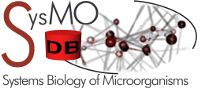
\includegraphics[width=6em]{res/sysmodb2.png}};
% % \node[scale=.7] (bmdb) at (9.9,3) {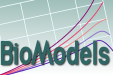
\includegraphics[width=5em]{res/bmdb.png}};
% % \node[scale=.7] (pmr2) at (8.1,3.3) {\includegraphics[width=4em]{res/CellML-eps-converted-to.pdf}};
% % \end{tikzpicture}
\end{frame}


\end{comment}



 
\begin{frame}{}{\mylogo}
	{\LARGE That's it!}\\[1.05em]
	%{\Large Want to talk? Drop me a message!}
	%{\LARGE Thanks for your attention!}
	\\[1.4em]
	
	
\includegraphics[height=1em]{res/github.pdf}\ 
	Fork me on GitHub\\
	\textcolor{colorscheme}{\url{https://github.com/FreakyBytes/bachelor-thesis}}
	
	
\includegraphics[height=1em]{res/twitter.png}
	\textcolor{colorscheme}{\tt\  \href{https://twitter.com/FreakyBytes}{@FreakyBytes}}\\
	
	
\includegraphics[height=1em]{res/XMPP_logo.pdf}
	\textcolor{colorscheme}{\tt\  martin@freakybytes.net}\\
	
	\includegraphics[height=0.8em]{res/mail.pdf}
	\textcolor{colorscheme}{\tt\  martin.peters4@uni-rostock.de} 
	
	
\end{frame}
	
	%\bibliography{ba-thesis.bib}
	\bibliography{zotero.bib}
	\bibliographystyle{apalike}
	
	\begin{appendix}
		\listoffigures
		
		\chapter*{Appendix}
		%% !TeX spellcheck = en_US

% some nice styling for code listings
\definecolor{mygreen}{rgb}{0,0.6,0}
\definecolor{mygray}{rgb}{0.5,0.5,0.5}
\definecolor{mymauve}{rgb}{0.58,0,0.82}

\lstset{ %
	backgroundcolor=\color{white},   % choose the background color; you must add \usepackage{color} or \usepackage{xcolor}
	basicstyle=\footnotesize,        % the size of the fonts that are used for the code
	breakatwhitespace=false,         % sets if automatic breaks should only happen at whitespace
	breaklines=true,                 % sets automatic line breaking
	captionpos=b,                    % sets the caption-position to bottom
	commentstyle=\color{mygreen},    % comment style
	deletekeywords={...},            % if you want to delete keywords from the given language
	escapeinside={\%*}{*)},          % if you want to add LaTeX within your code
	extendedchars=true,              % lets you use non-ASCII characters; for 8-bits encodings only, does not work with UTF-8
	frame=no,	                   % adds a frame around the code
	keepspaces=true,                 % keeps spaces in text, useful for keeping indentation of code (possibly needs columns=flexible)
	keywordstyle=\color{blue},       % keyword style
	language=Octave,                 % the language of the code
	otherkeywords={*,...},           % if you want to add more keywords to the set
	numbers=left,                    % where to put the line-numbers; possible values are (none, left, right)
	numbersep=5pt,                   % how far the line-numbers are from the code
	numberstyle=\tiny\color{mygray}, % the style that is used for the line-numbers
	rulecolor=\color{black},         % if not set, the frame-color may be changed on line-breaks within not-black text (e.g. comments (green here))
	showspaces=false,                % show spaces everywhere adding particular underscores; it overrides 'showstringspaces'
	showstringspaces=false,          % underline spaces within strings only
	showtabs=false,                  % show tabs within strings adding particular underscores
	stepnumber=2,                    % the step between two line-numbers. If it's 1, each line will be numbered
	stringstyle=\color{mymauve},     % string literal style
	tabsize=2,	                   % sets default tabsize to 2 spaces
	title=\lstname                   % show the filename of files included with \lstinputlisting; also try caption instead of title
}

% helper for importing csv files with underscores
\DeclareUrlCommand\UScore{\urlstyle{rm}}
\newcommand{\expUScore}{%
	\expandafter\expandafter\expandafter
	\UScore
	\expandafter\expandafter\expandafter
}

\chapter{Simple demo \sbml models}
\section{Simple demo SBML version1}
\label{sec:appendix:simple-demo:v1}
\lstinputlisting[language=XML]{../supplementary/demo-sbml-simple/version1.xml}

\section{Simple demo SBML version2}
\label{sec:appendix:simple-demo:v2}
\lstinputlisting[language=XML]{../supplementary/demo-sbml-simple/version2.xml}

\chapter{Render of Delta between a more advanced demo model}
\begin{figure}[h]
	\centering
	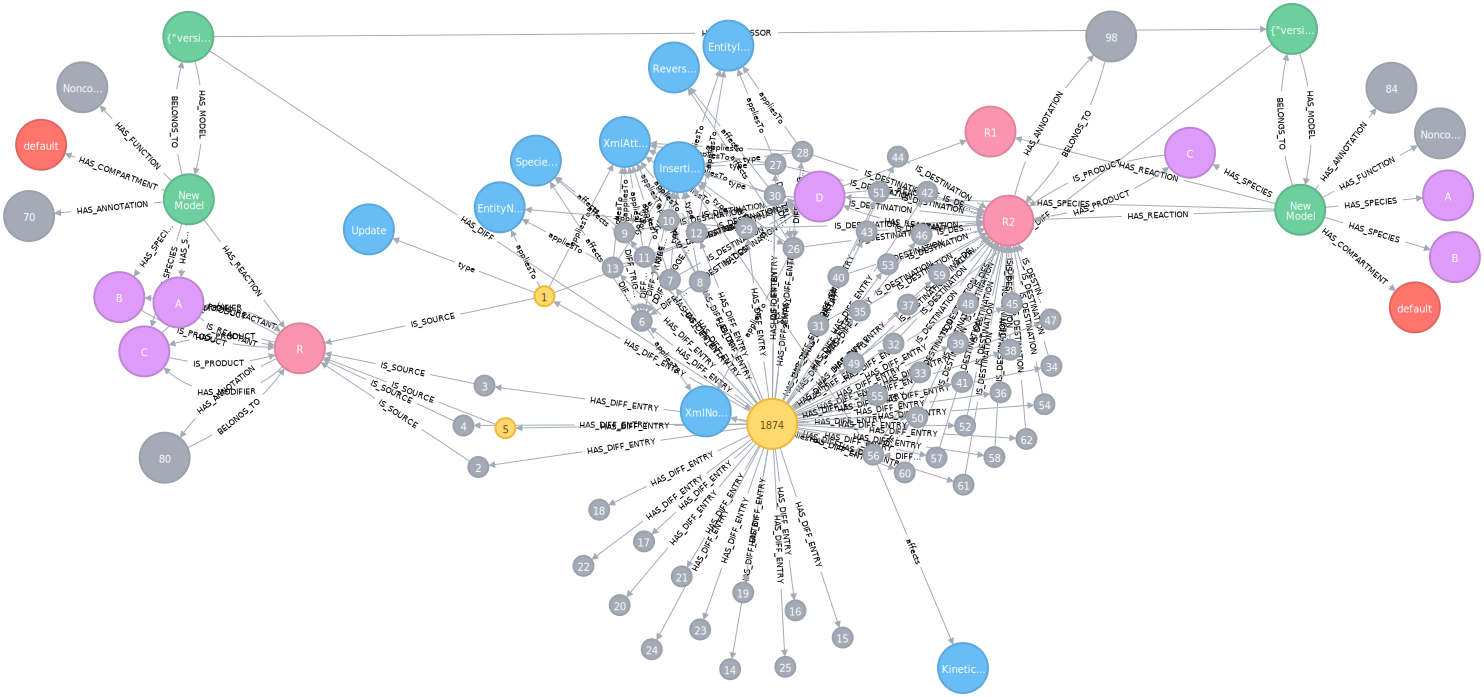
\includegraphics[width=\textwidth]{resources/neo4j-renders/demo-sbml-diff.pdf}
	\caption{\neoj graph representation of a delta between two demo models}
	\label{fig:appendix:demo-sbml-diff}
\end{figure}

\chapter{Representation of \comodi in \masymos}
\begin{figure}[h]
	\centering
	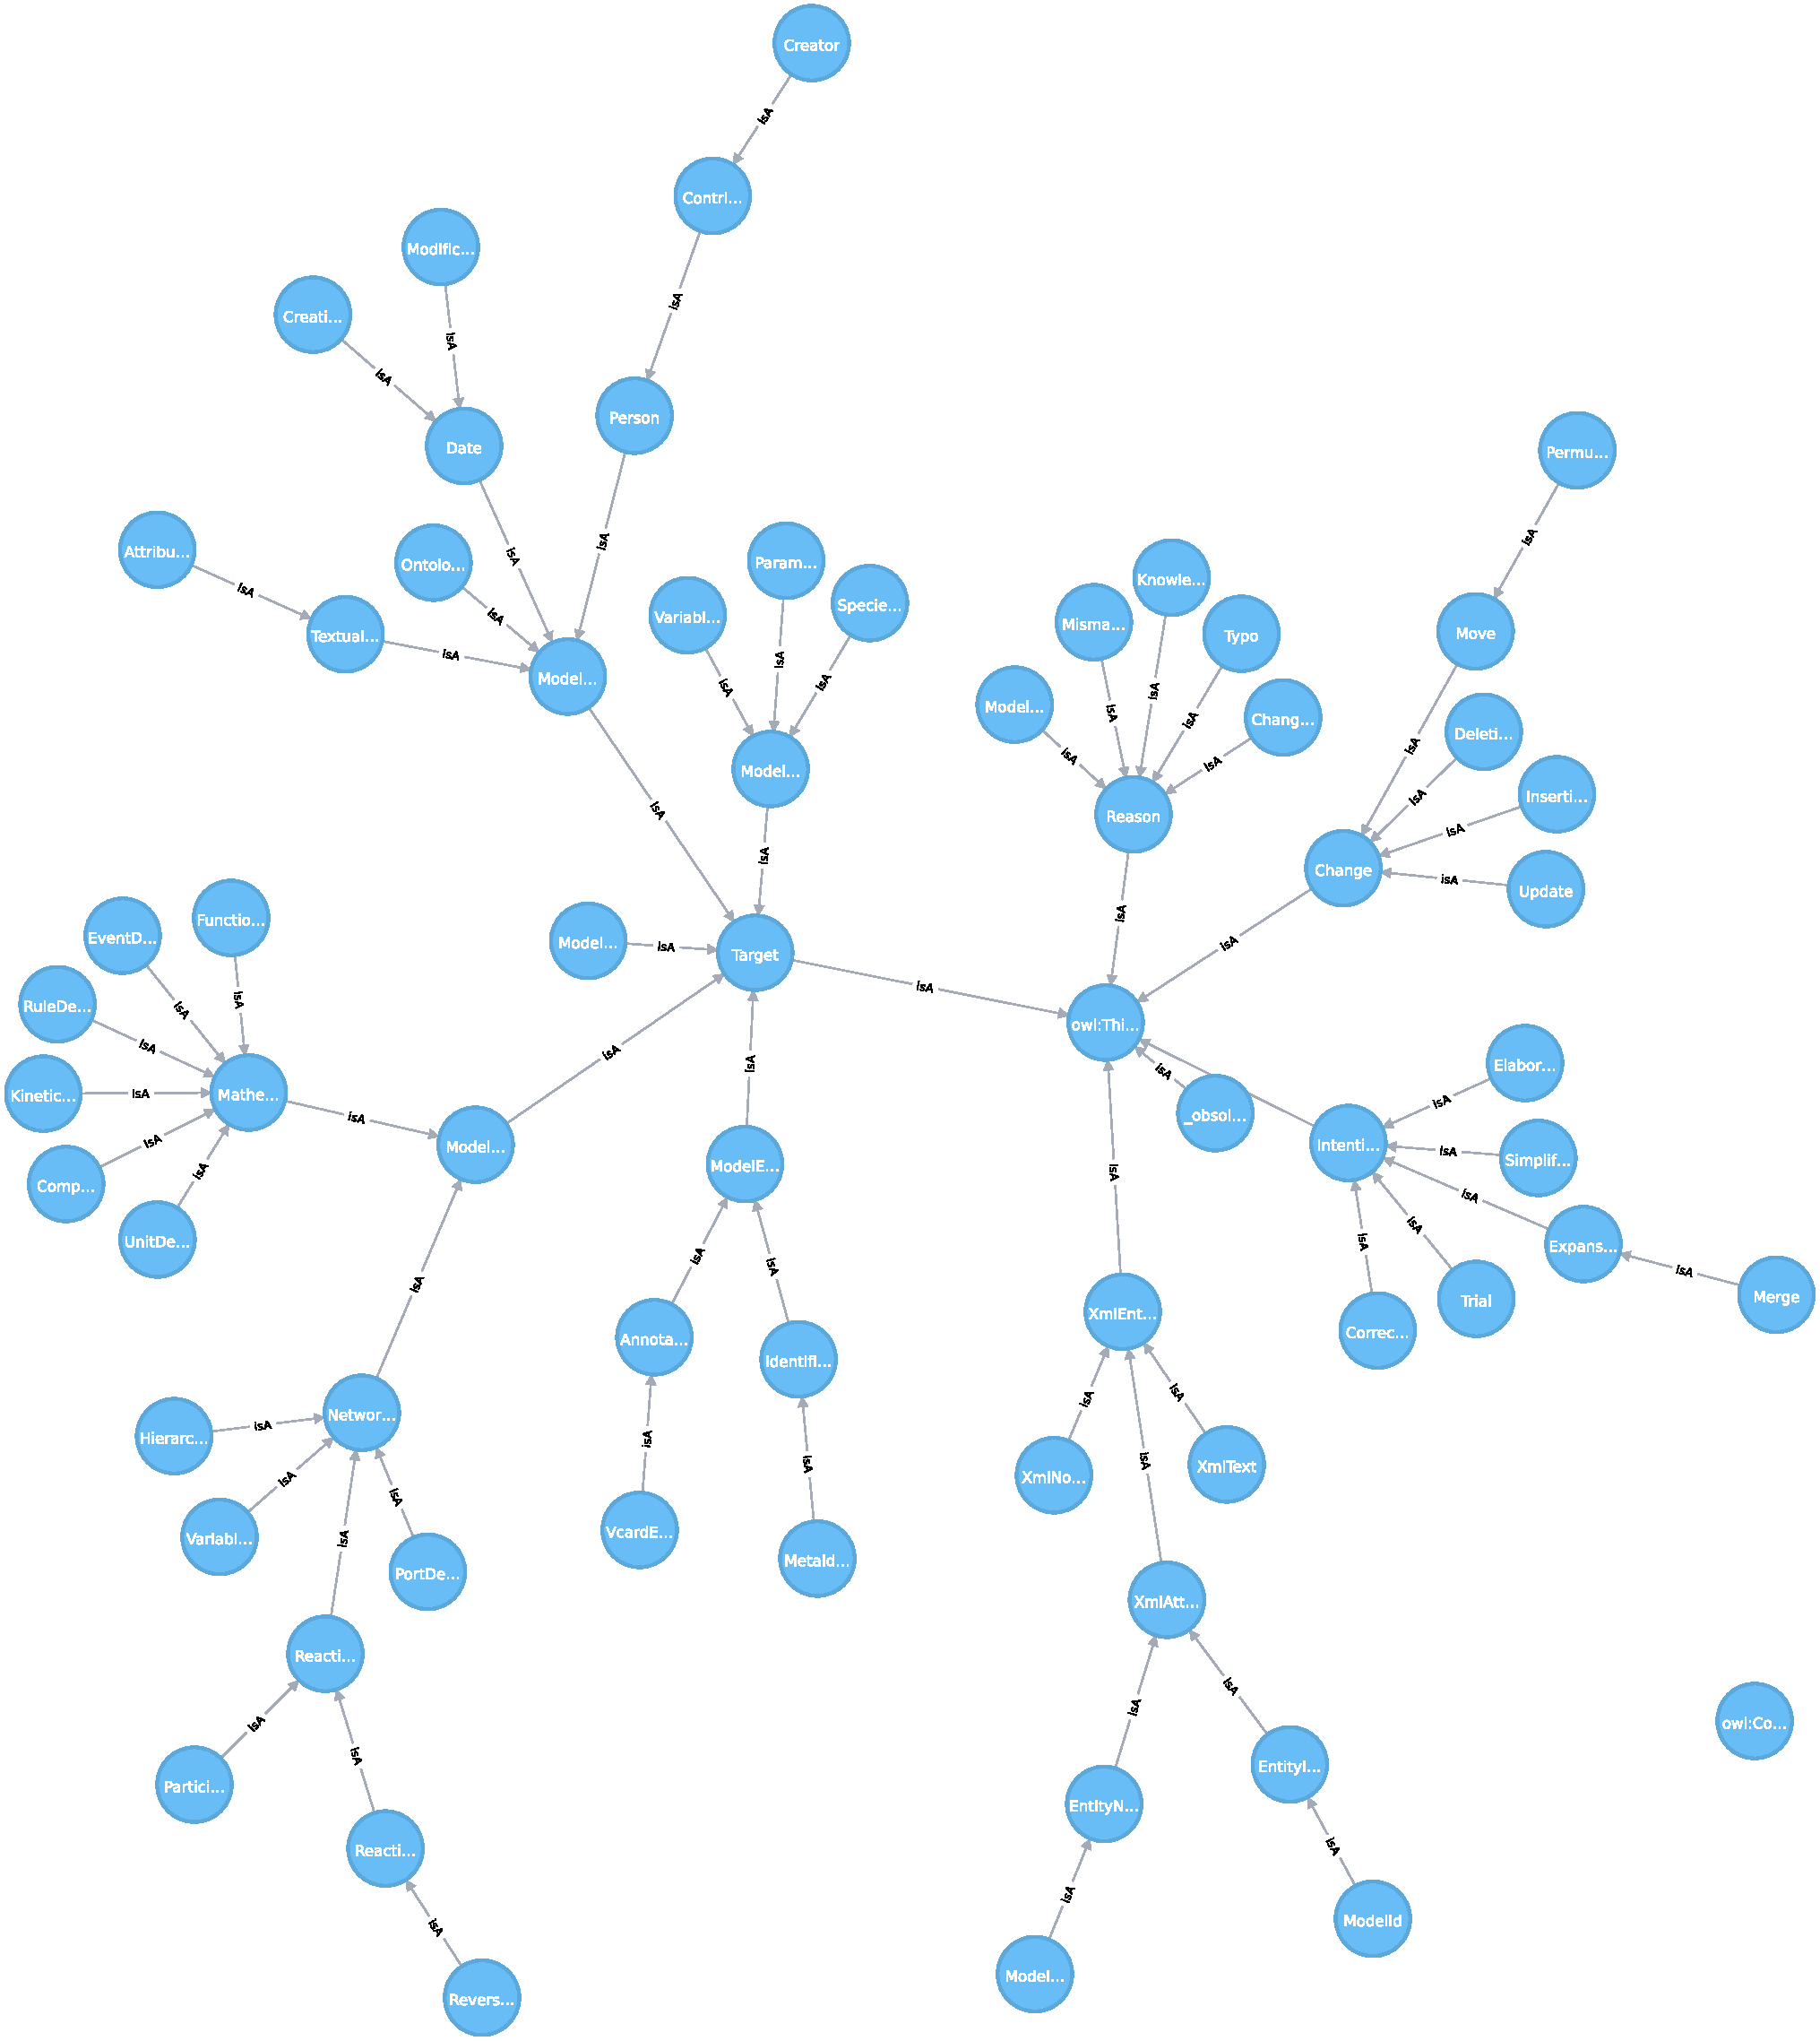
\includegraphics[width=\textwidth,height=0.5\textheight,keepaspectratio]{resources/neo4j-renders/comodi.pdf}
	\caption{Representation of \comodi in \masymos/\neoj}
	\label{fig:appendix:neo4j-comodi}
\end{figure}

\chapter{Overview of Node- and Relationship types}
\todo{tables are ugly as hell...}
\todo{write introduction thingy, where these numbers are coming from}

\section{Graphical Overview}
\begin{figure}[H]
	\centering
	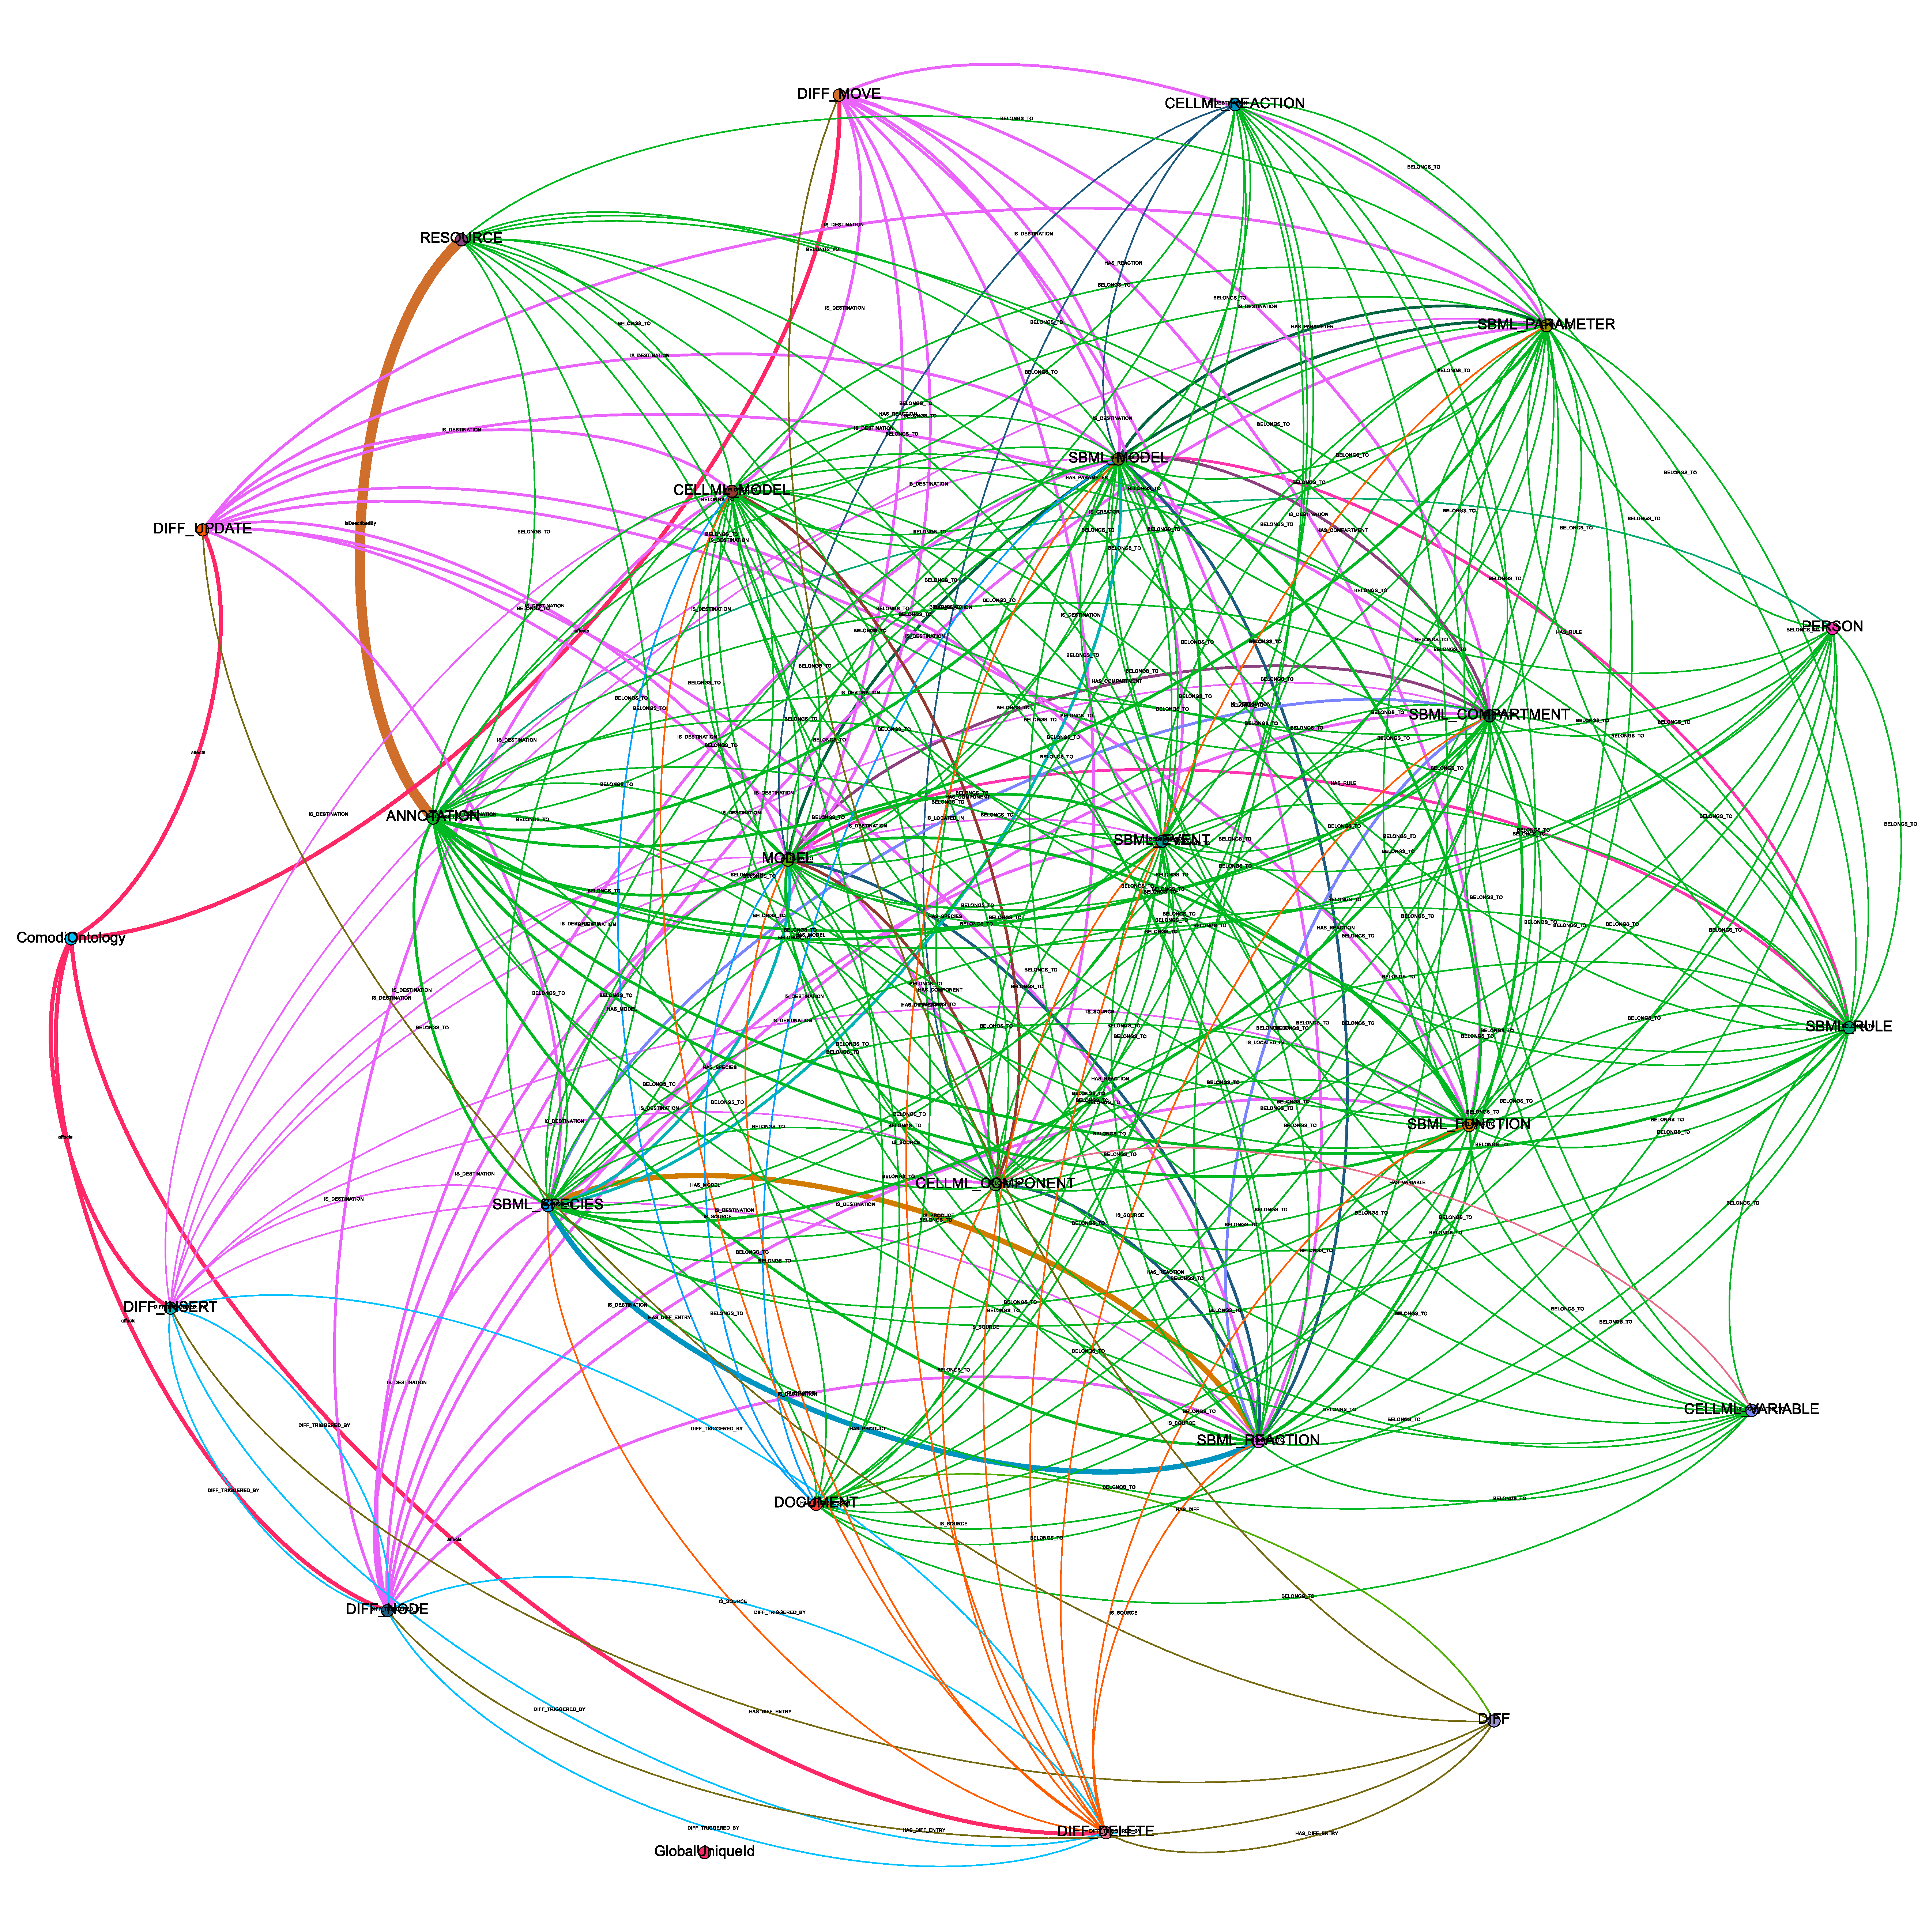
\includegraphics[width=\textwidth,height=0.5\textheight,keepaspectratio]{resources/neo4j-renders/large-test-meta-graph.pdf}
	\caption{Overview of all used node types and relations between them}
	\label{fig:appendix:meta-graph}
\end{figure}

\section{List of all used Node types}
\begin{longtable}{ l r }
	\hline \bfseries Node Label & \bfseries No. of occurrence \\\hline \endhead
	\csvreader[head to column names]{resources/neo4j-renders/large-test-meta-graph-nodes.csv}{} %
	{\expUScore{\label} & \count \\} %
	%\hline
\end{longtable}

\section{List of all used Relationship types}
\begin{longtable}{ l c r r }
	\hline \bfseries Source Node Label & \bfseries Relationship Type & \bfseries Destination Node Label \\\hline \endhead %
	\csvreader[]{resources/neo4j-renders/large-test-meta-graph-edges-expanded.csv}{Source=\sourceNode,Target=\targetNode,label=\relLabel,count=\count} %
	{\expUScore{\sourceNode} & \expUScore{\relLabel} & \expUScore{\targetNode}\\} %
	%\hline
\end{longtable}

	\end{appendix}
\end{document}
